\begin{quote}
	\textit{``The sinister thing about a simstim construct, really, was that it carried the suggestion that any environment might be unreal, that the windows of the shopfronts she passed now with Andrea might be figments.''}
\end{quote}
\hfill \textit{Count Zero, William Gibson}
\\
\\

%=========================================================================================================
%=========================================================================================================

\label{chapter-vtw}

This chapter recounts the development of the Virtual Time Window, a platform that endeavoured to explore the suitability of a familiar alternate reality modality of interaction, using a tablet computer, GPS, accelerometer and magnetometer in combination with a Second Life/OpenSim based virtual environment, for investigation into the parallel reality concept. Virtual heritage is introduced as a field with a history of successful applications of alternate reality technologies and to which parallel reality promises to be of further benefit. The Virtual Time Window platform was tested within such a scenario, to explore the ruins of a 14th century cathedral in tandem with a complete virtual reconstruction of it as it stood in its prime.

%=========================================================================================================

\section{Virtual Heritage}

Alternate reality technologies have been used for over two decades~\cite{Roussou2002} to aid in the investigation, understanding and dissemination of information pertaining to our past in the fields of archaeology and cultural heritage. Whilst archaeology studies human activity through the recovery of remains, heritage is concerned also with intangible attributes of society; tradition, art, narratives and other cultural evidences~\cite{Roussou2002}. \textit{Virtual heritage} is the name given to the application of advanced imaging techniques, including alternate realities, to the synthesis, conservation, reproduction, representation, reprocessing and display of this cultural evidence~\cite{roussou:photorealism}.

These techniques provide access to locations and artefacts scattered about the world which may reside in private collections inaccessible to scholars, much less to the general public, and outwith their original context of creation~\cite{griffin:recovering}. They allow recreations to be made of the numerous cultural heritage objects that are deteriorating or are at risk of being lost, whether due to natural causes such as weather and natural disasters or due to acts of man such as civil war~\cite{Ikeuchi2003}.

Virtual heritage techniques offer substantial benefits to collaborative investigation of heritage sites, providing multiple users with the ability to collaborate via a multitude of different visualization modalities including video see-through head-tracked HMDs, projected table surfaces, large screen displays and tracked hand-held displays, including the ability for experts physically located at a particular site to collaborate with those remote to it~\cite{benko:collaborative}. This combination of different techniques not only benefits experts, but has been used in the creation of contiguous platforms for building and managing exhibitions of 3D models of artefacts accessed in museums, galleries and via the Web~\cite{Wojciechowski2004}, focussed not only on the digitization and subsequent interaction with such content to aid in its preservation and protection, but also with making these resources as widely available as possible to any interested parties (scientists, archaeologists, curators, historians and the general public)~\cite{walczak:applications}.

Even traditionally two-dimensional visual resources associated with cultural heritage can be integrated into such state-of-the-art systems, visualized via immersive CAVE (Cave Automatic Virtual Environment~\cite{Tzortzaki2002}) techniques as part of `information landscapes'~\cite{Ruffaldi2008}. Virtual heritage techniques such as these are of particular benefit to young people as cultural heritage sites often arouse little involvement in them, especially if the site's present day appearance bears few traces of its original stature and makes it difficult to appreciate its original splendour and importance~\cite{ardito:combining}.

%=========================================================================================================

\subsection{Alternate Reality Techniques in Virtual Heritage}

Due to the diverse approaches that have been used in the application of visualization techniques to the cultural heritage sector, attempting to comprehensively list them is impractical. Comparison via a taxonomical model that classifies approaches according to various characteristics is thus the approach adopted by Papagiannakis et al.~\cite{Foni2010} who produced the taxonomical space shown by figure \ref{taxonomy_1.png}.

\begin{figure}[h]
\centering
  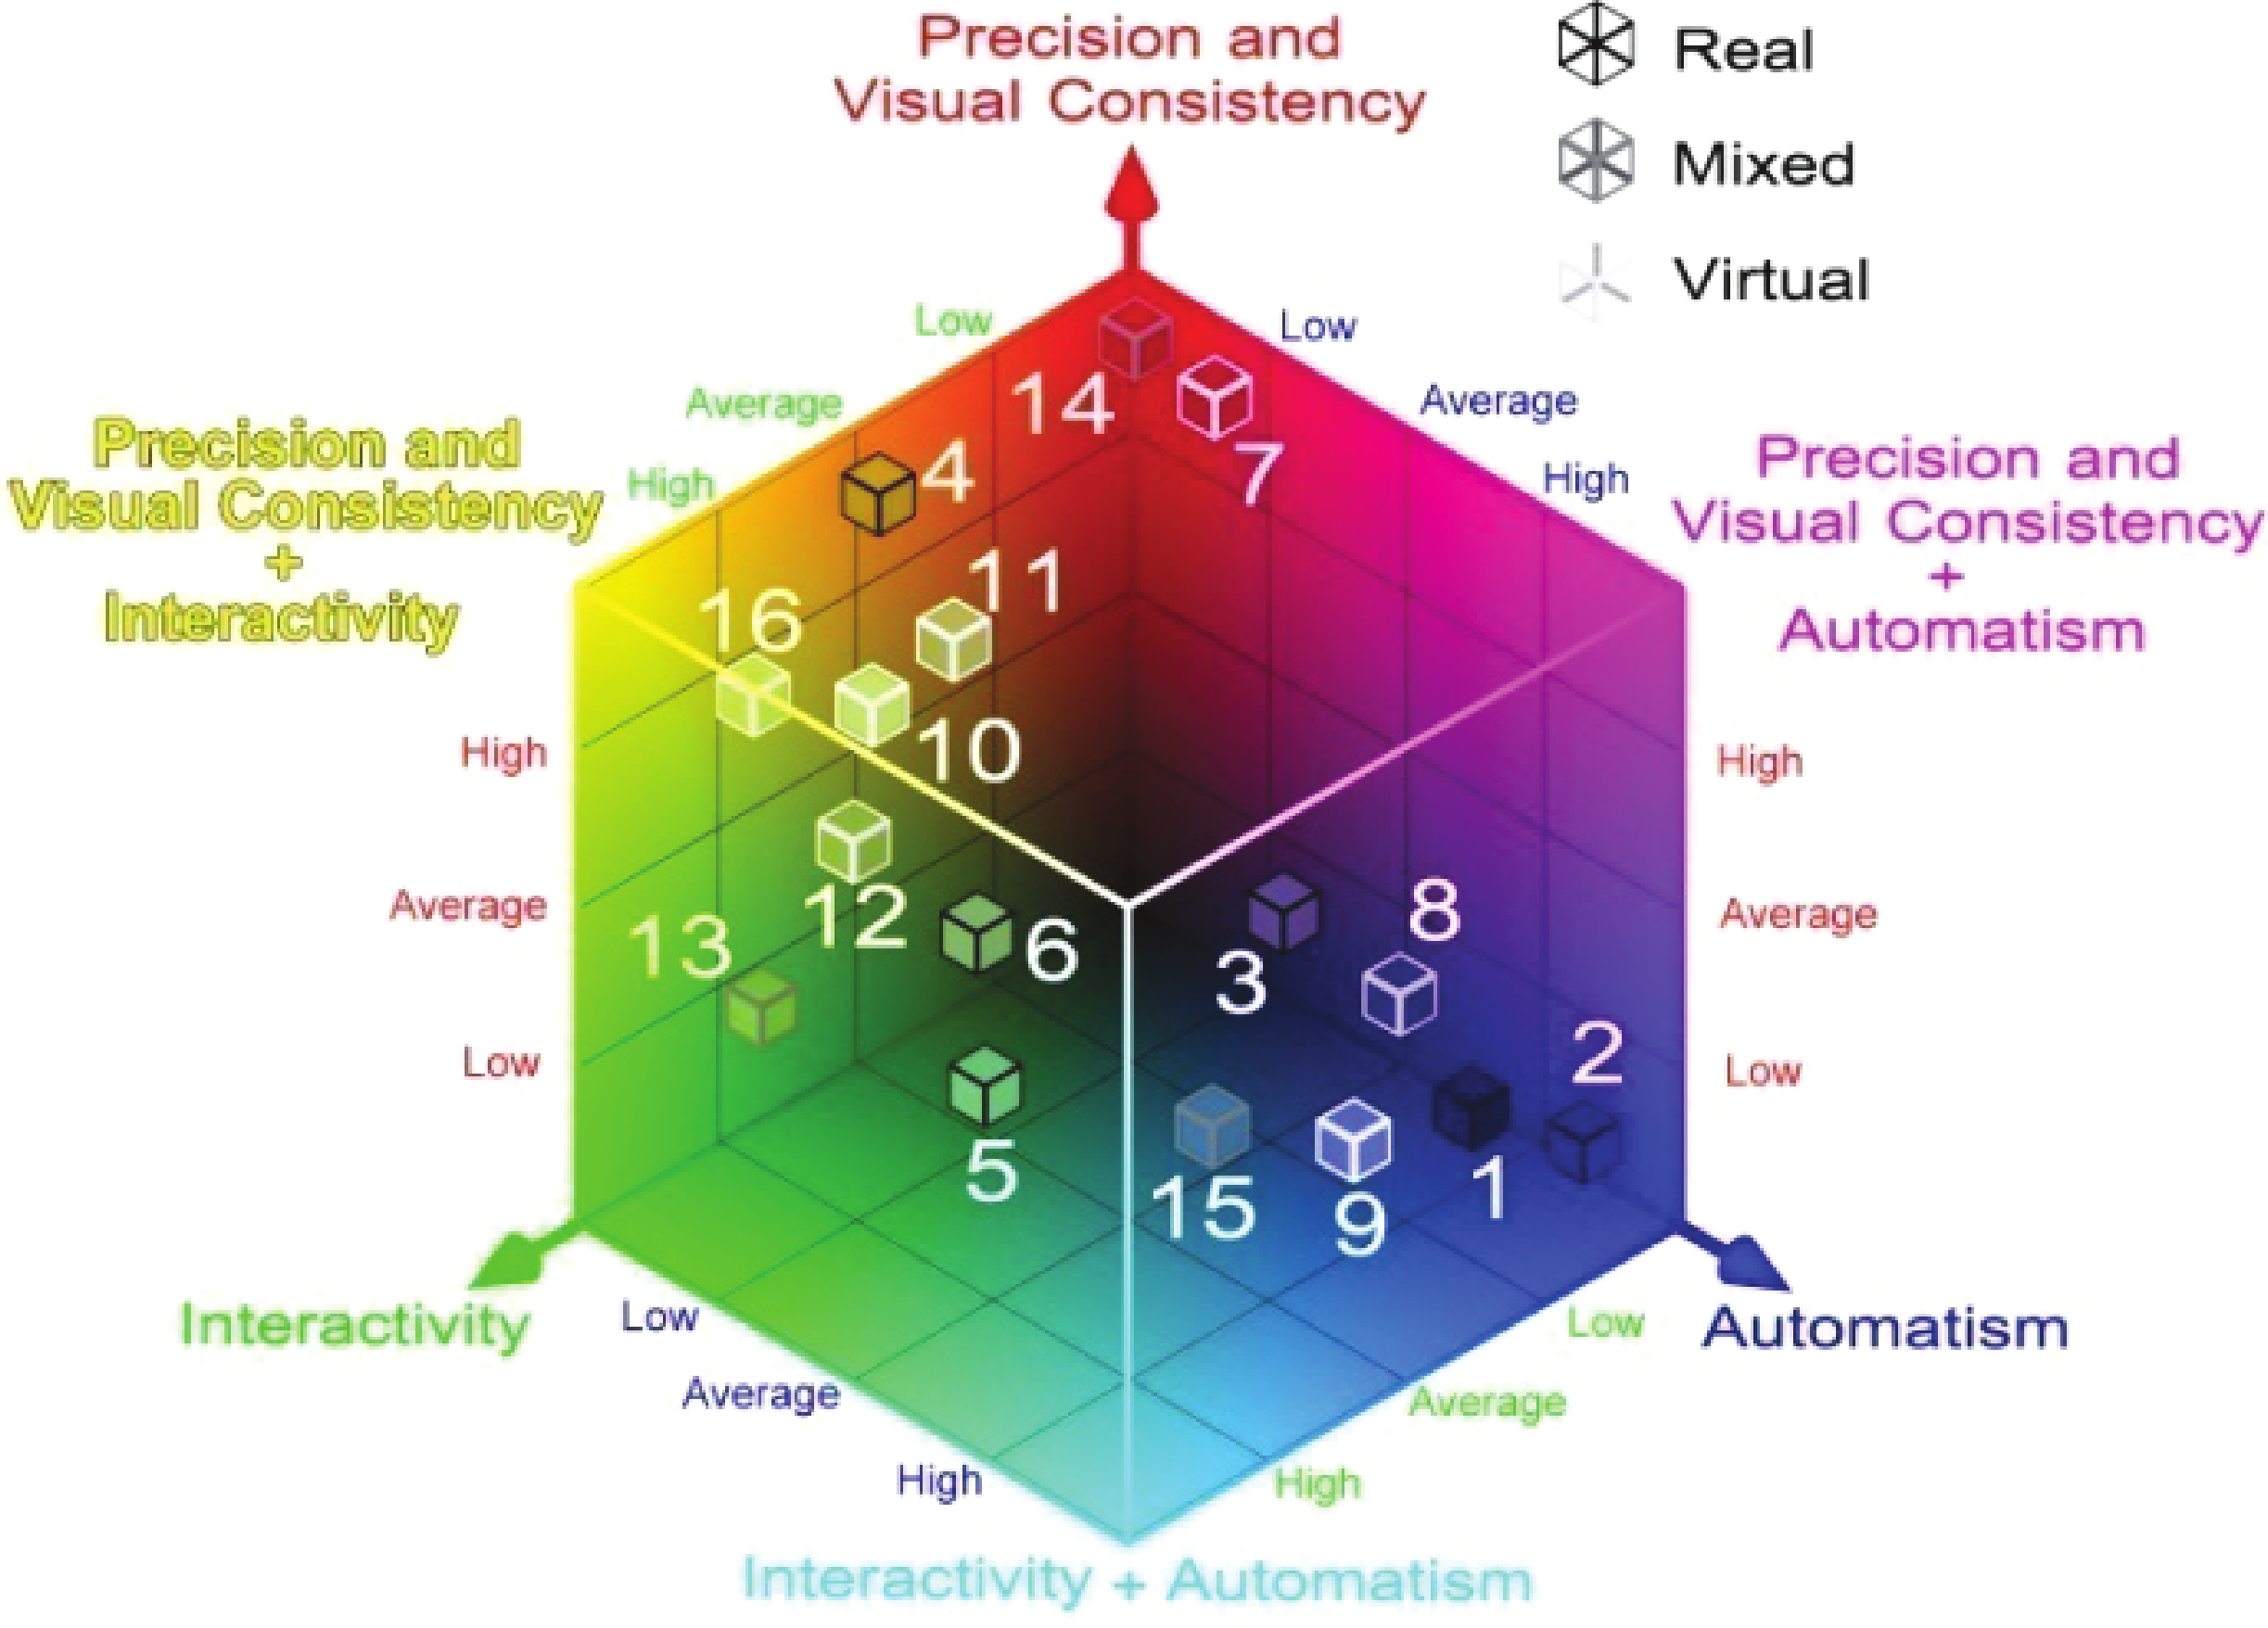
\includegraphics[width=.7\linewidth]{taxonomy_1.png}
  \caption{Taxonomical space of visualization strategies used in cultural heritage~\cite{Foni2010}, image courtesy George Papagiannakis.}
  \label{taxonomy_1.png}
\end{figure}

This model classifies visualization strategies according to four continua, represented by the three physical dimensions of the cube and the degree of shading of each point within the cube. The x axis represents the level of automatism, which refers to the span of the development cycle required to produce the visualization; the y axis represents the level of precision, referring not only to the amount of geometrical detail but to all elements that can contribute to or enhance reliability; and the z axis represents the level of interactivity, defined in this context as:

\begin{quote}
	\textit{``\ldots its capacity to contextually offer the possibility to subjectively experience an interactive behaviour in a synchronous way, thus enabling the user the opportunity to meaningfully contribute to a given experience or to affect in real time the visualized  item''}~\cite{Foni2010}.
\end{quote}

The shading of each point within the cube represents its degree of virtuality, conceptually analogous to Milgram and Kishino's reality-virtuality continuum (see section \ref{milgram&kishino}) with real world/world unmodelled represented as solid black, virtual reality/world completely modelled as completely white and positions in-between as various shades of grey. Papagiannakis et al. explain the position of 16 visualization techniques applied to cultural heritage, including both traditional techniques and state-of-the-art methodologies, by their positions within the cube and via the table included as figure \ref{taxonomy_2.png}.

\begin{figure}[h]
\centering
  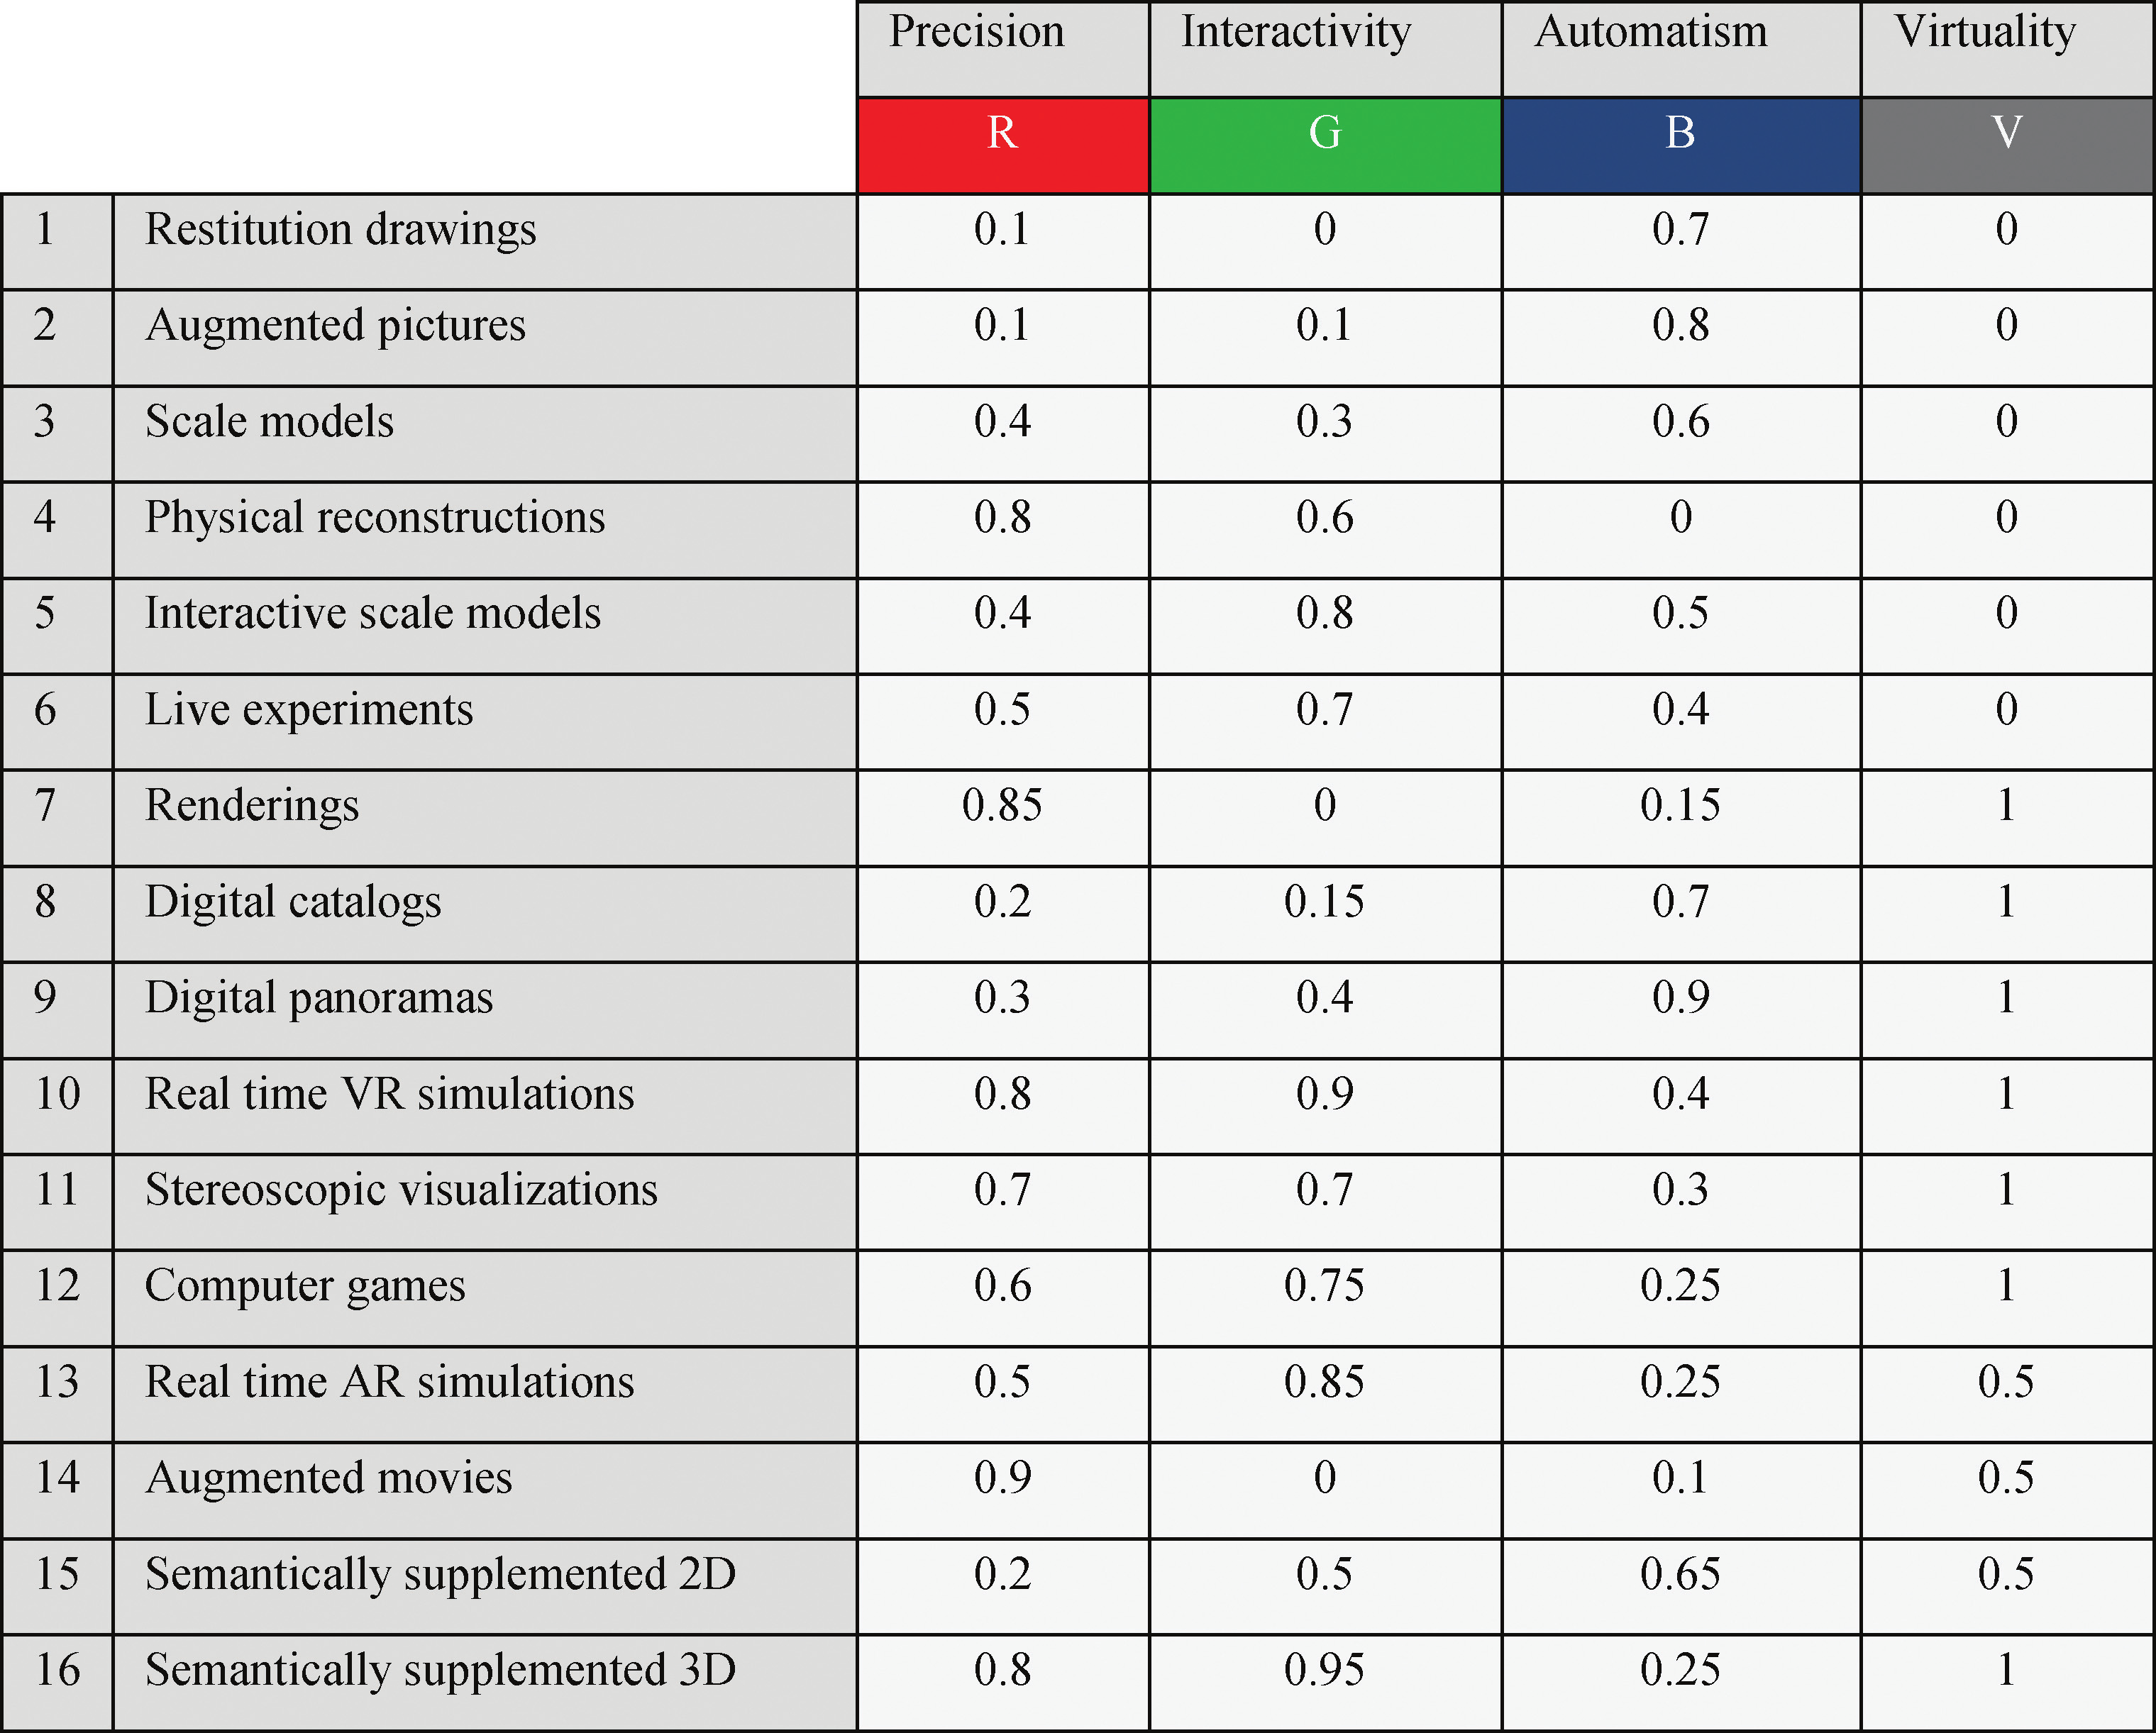
\includegraphics[width=.8\linewidth]{taxonomy_2.png}
  \caption{Coordinate sets for each approach within the taxonomical space of figure \ref{taxonomy_1.png} ~\cite{Foni2010}, image courtesy George Papagiannakis.}
  \label{taxonomy_2.png}
\end{figure}

%=========================================================================================================

\subsection{Existing Virtual Heritage Applications}
\label{existing-virtual-heritage-applications}
In terms of alternate reality techniques, real time augmented reality simulations (category 13 of figures \ref{taxonomy_1.png} and \ref{taxonomy_2.png}) have been used to add artefacts, actors and reconstructed architecture to views of present day sites that are still accessible and may bear traces of their original status, whilst real time virtual reality simulations (category 10) have been used to host more complete reconstructions of entire buildings and settlements for interaction via screen, HMD and CAVE, including where the present day site bears no evidence of its past status or is inaccessible due to latter development, change in landscape, etc.

%=========================================================================================================

The ARCHEOGUIDE project (Augmented Reality-based Cultural Heritage On-site GUIDE)~\cite{vlahakis:archeoguide} aimed to provide a \textit{``personalized electronic guide and tour assistant''} to cultural heritage site visitors. On-site help and augmented reality reconstructions of on-site ruins were presented via a laptop, a tablet computer and a PDA, using GPS for location tracking and magnetometer to ascertain direction such that augmentations could be placed accordingly. The applications supported by the platform range from archaeological research to education, multimedia publishing and cultural tourism. The platform was prototyped at the archaeological site of Olympia, Greece.

As well as being used for walking tours, augmented reality has been combined with the concept of telepresence to create `augmented telepresence', allowing participants to experience a `fly-through' of the ancient Nara Heijo-kyo capital of Japan, by combining aerially captured omnidirectional video with related information using augmented reality techniques~\cite{Okura2006,Okura2011}.

Augmenting views of the real world with real-time animated virtual humans has been explored by several projects, including the LIFEPLUS EU IST project which aimed to produce \textit{``an innovative 3D reconstruction of ancient frescos-paintings through the real-time revival of their fauna and flora, featuring groups of virtual animated characters with artificial life dramaturgical behaviors, in an immersive augmented reality environment''}~\cite{Papagiannakis2004}. This project pushed established augmented reality applications in the field by exploring narrative design in fictional spaces, with the aim of increasing immersion via realistic interaction, making use of captured/real-time video of a real scene, presenting the visitor with \textit{``an immersive and innovative multi-sensory interactive trip to the past''}~\cite{Papagiannakis2005}. These realistic simulations of animated virtual human actors were employed in a mobile and wearable setup, in abandonment of traditional concepts of static cultural artefacts or rigid augmentations of real world features, making use of a markerless camera tracker and mixed reality illumination model for more consistent real-virtual and virtual-real rendering. This platform was demonstrated in a case study on the real site of ancient Pompeii and whilst initially targeted at the cultural heritage sector, the authors clarify that as a platform it is not limited to these subjects~\cite{Papagiannakis2007}. This concept of extending rigid and static augmented reality with character-based event representations hopes to recreate not just discrete artefacts but the entirety of `daily life' at the scene~\cite{Papagiannakis2009}.

Although many applications of augmented reality to cultural heritage sites are mobile in nature, using a variety of tracking techniques to localise the user and determine their orientation, including GPS~\cite{vlahakis:archeoguide}, visual tracking of robust features of the environment~\cite{Kim2009} and omnidirectional range sensing of a landmark database~\cite{Taketomi2011}, there are also those that present a static interface~\cite{Weng2012} similar to the coin-operated binoculars and telescopes commonly found at popular tourist attractions.

%=========================================================================================================

VR has been used in virtual heritage not only where the real site is no longer accessible, too remote or does not bear any similarity to its original status, but also to allow for more effective control over the atmospheric qualities of the environment being recreated; effects such as fog, sky, water and particles can be effected, exploiting the latest graphical hardware by making use of shaders to deliver high quality graphics~\cite{deamicis:gamebased}. The use in virtual heritage of a HMD or CAVE that completely blocks stimuli from the user's real world surroundings~\cite{cabral:x3dexperience,Christou2006}, which can be situated at the site itself and create a `space of illusion'~\cite{Tzortzaki2002}, allows for this complete level of control. Unless an augmented reality system employs various environmental monitoring techniques, the augmentations that it overlays upon the user's view of the real world will often have differing illumination than their real surroundings which has a detrimental effect upon their perceived realism~\cite{mcnamara:lightness}.

Whereas many heritage representations, architectural walkthroughs and simulations of artefacts and places have defined a practice where photorealism is considered an important measure of the representation's success, there is an argument that whilst such an emphasis on realism and historical accuracy and authenticity is important, such photorealistic methods can limit the flexibility of reconstructions with regards to how much they can be modified and altered to explore different reconstruction hypotheses~\cite{roussou:photorealism}. Emphasis upon photorealistic graphical quality also has considerations when it comes to real time performance and many intelligent techniques may need to be employed to maintain acceptable performance as complexity of reconstructions increases~\cite{willmott:largecomplex} and it is not uncommon for VR systems to \textit{``reduce realism in order to achieve the desired real time performance''}~\cite{Chalmers2014}. Particularly for dissemination to the general public in museums and visitor centres, performance is often considered more important than historical accuracy, a trait that mirrors a common theme in the computer gaming industry where \textit{``compelling action can reduce the need for full-scale visualization''}~\cite{Heim2014} because \textit{``abstraction can be just as engaging to users as a sense of realism''}~\cite{Champion2014}.

%=========================================================================================================

\subsection{Situated Simulation}
\label{situated-simulation}
One application of alternate reality techniques to the field of cultural heritage that warrants particular attention is that of `situated simulation' (sitsim)~\cite{Liestøl2009}. Since 2009 Liest\o l et al. have investigated the use of smartphones, and later tablets, for presenting visitors to cultural heritage sites with Unity based 3D reconstructions, using the location and orientation sensors built into the devices to appropriately move the virtual vantage as the user moves around the site.

\begin{quote}
	\textit{``When using a situated simulation there is then approximate identity between the user’s visual perspective and perception of the real physical environment, and the user’s perspective in(to) the virtual environment as this is audiovisually presented by means of the phone and sitsim’s interface. The relative congruity between the `real' and the `virtual' is obtained by allowing the camera’s position, movement and orientation in the 3D environment, to be constrained by the orientation- and location technology of the smartphone: As the user moves the phone in real space the perspective inside the virtual space changes accordingly.''}~\cite{Liestøl2011}
\end{quote}

These sitsim systems have been labelled by their creators as examples of `indirect augmented reality', a concept introduced by Wither at al.~\cite{Wither2011} to alleviate the dependency of traditional augmented reality systems upon highly accurate position and orientation data in order to successfully place virtual objects at the correct position upon camera feeds of the real world scene. Indirect augmented reality forgoes a live camera feed of the real environment in place of previously captured panoramic photographs. Knowing the exact position at which the photographs were captured allows for zero registration error between virtual objects and the photographs, moving the registration error to the edges of the device's screen where the photographs meet the real environment from which they were captured. The effect is to improve the perceived quality of registration between virtual objects and real background, as registration error at the screen's edges is perceived as being `better' than between virtual objects and real background within the screen, in a similar manner as to how parallel reality was posited in section \ref{caseforpr} as having relaxed registration requirements over augmented reality implementations.

\begin{quote}
	\textit{``Moving registration error to the edge of the screen is better in part because it is a more difficult place to detect error due to both the bezel around the screen, and the altered field-of-view parameters of the on-screen image. In many ways, people are also already trained to believe that when they see a view of the real world on the screen of the mobile device it lines up with the world behind it. This is largely due to the proliferation of digital cameras already using the screen as a viewfinder.''}~\cite{Wither2011}
\end{quote}

However likening the Unity based virtual environments of sitsim systems to the panoramic photographs of indirect augmented reality does not fit well with the definition of augmented reality adopted in table \ref{adopted-alternate-reality-definitions} and undervalues the novelty of sitsim as a concept. Fundamentally the indirect augmented reality platforms presented by Wither et al. still present the user, via the screen of the device, with a view of the real environment upon which virtual objects are placed, even though that view of the real environment is no longer `live' but is instead a photograph captured at a previous point in time. The sitsim platforms presented by Liest\o l et al. however, present via the screen of the device a view of a complete virtual environment rather than a mediated and augmented image of the real environment.

Whilst one could argue that the experience of using a sitsim platform is similar to that of an indirect augmented reality platform, even if it is the human mind that is ultimately performing the `mixing' of the virtual environment with the real environment whilst in a `true' indirect augmented reality platform the mixing of virtual objects and real environment is performed upon the device, a distinction should be made to appreciate that a sitsim system nonetheless presents users with two complete environments, one real and the other virtual, rather than a single environment consisting of a real primary environment augmented by virtual objects. This distinction was raised by Liest\o l et al. and visualised upon the reality-virtuality continuum in figure \ref{sitsim-1.png} (compare this with the explanation of parallel reality in section \ref{positionofcrossreality} around figure \ref{virtuality-continuum-cross-reality-1}). Furthermore Liest\o l speaks of how sitsim creates \textit{``double perspective''}~\cite{Liestøl2009}, allowing presentation of topics and subject matters absent or invisible in the real world, wherein the user performs \textit{``oscillations between \ldots\ double descriptions''}~\cite{Liestøl2014}, further alluding to the notion of two complete environments that the user switches their attention between.

\begin{figure}[h]
\centering
  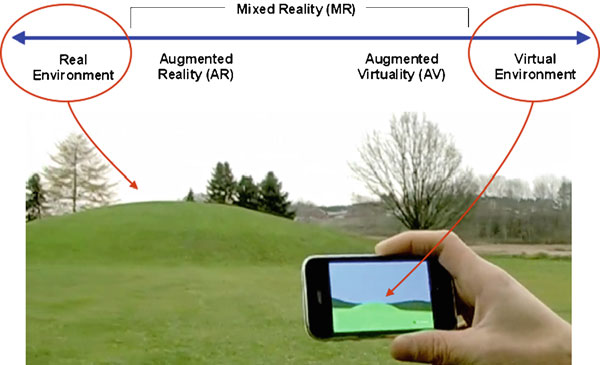
\includegraphics[width=.6\linewidth]{sitsim-1.png}
  \caption{The two complete environments of a sitsim platform~\cite{Liestøl2011}, with kind permission from Springer Science and Business Media.}
  \label{sitsim-1.png}
\end{figure}

In recognising this distinction a platform in the style of sitsim represents a potential basis for investigation of the parallel reality concept in scenarios with high spatial equivalence; indeed, Liest\o l's notion of `approximate identity' and the use of the term `situated' in the concept's title would seem to directly relate to the concept of spatial equivalence introduced in section \ref{spatial-equivalence}. Considering sitsim as spatially equivalent parallel reality instead of as indirect augmented reality would also avoid the somewhat confusing visualisation from Liest\o l et al. of sitsim occupying a region of the reality-virtuality continuum that falls within the realm of augmented reality but whilst simultaneously being outwith the region of mixed reality~\cite{Liestøl2011}.

%sitsim-2.png

%=========================================================================================================

\subsection{Virtual Heritage at the University of St Andrews}

\label{virtual-heritage-at-st-andrews}

%\textbf{***Include references to Kris Getchell's thesis? Experiential learning, etc?}

The Open Virtual Worlds (OVW) research group at the School of Computer Science at the University of St Andrews has been employed in virtual heritage projects since 2007~\cite{Getchell2007}, producing a number of reconstructions of cultural heritage sites around Scotland and further afield. These reconstructions have been produced through collaborations with academics from the university's Art History, History and Archaeology departments, as well as with domain experts from heritage organisations including Historic Scotland\footnote{\url{http://www.historic-scotland.gov.uk/}} and the National Trust for Scotland\footnote{\url{http://www.nts.org.uk/}}. These projects range from a reconstruction of a small church to much larger reconstructions such as that of the cathedral at St Andrews, which represents several years of work~\cite{Kennedy2013}. Whilst the cathedral reconstruction was completed as a research project, other reconstructions were produced specifically for use in schools in Scotland (including Linlithgow palace shown in figures \ref{linlithgow_real.jpg} and \ref{linlithgow_reconstruction.png}), others for outreach purposes (including Mosfell Viking farmstead in Iceland shown in figures \ref{mosfell_outside.jpg} and \ref{mosfell_inside.jpg}) and still others were built specifically for installation into museums (including Caen Township shown in figure  \ref{caen_township_outside.jpg}). Some of these reconstructions are inhabited with virtual humans that are scripted to perform certain actions specific to the role they depict at the site (virtual humans in the cathedral model are shown in figures \ref{cathedral_npc_standing.png} and \ref{cathedral_npc_talking.png}).

\TwoFig{linlithgow_real.jpg} {Linlithgow Palace today.} {linlithgow_real.jpg}
       {linlithgow_reconstruction.png} {Linlithgow Palace reconstruction.} {linlithgow_reconstruction.png}

\TwoFig{mosfell_outside.jpg} {Mosfell Viking Longhouse reconstruction (exterior).} {mosfell_outside.jpg}
	   {mosfell_inside.jpg} {Mosfell Viking Longhouse reconstruction (interior).} {mosfell_inside.jpg}

%\TwoFig{caen_township_outside.jpg} {Caen Township reconstruction.} {caen_township_outside.jpg}
%       {caen_township_inside_wireframe.jpg} {Caen Township reconstruction wireframe detail.} {caen_township_inside_wireframe.jpg}

\begin{figure}[h]
\centering
  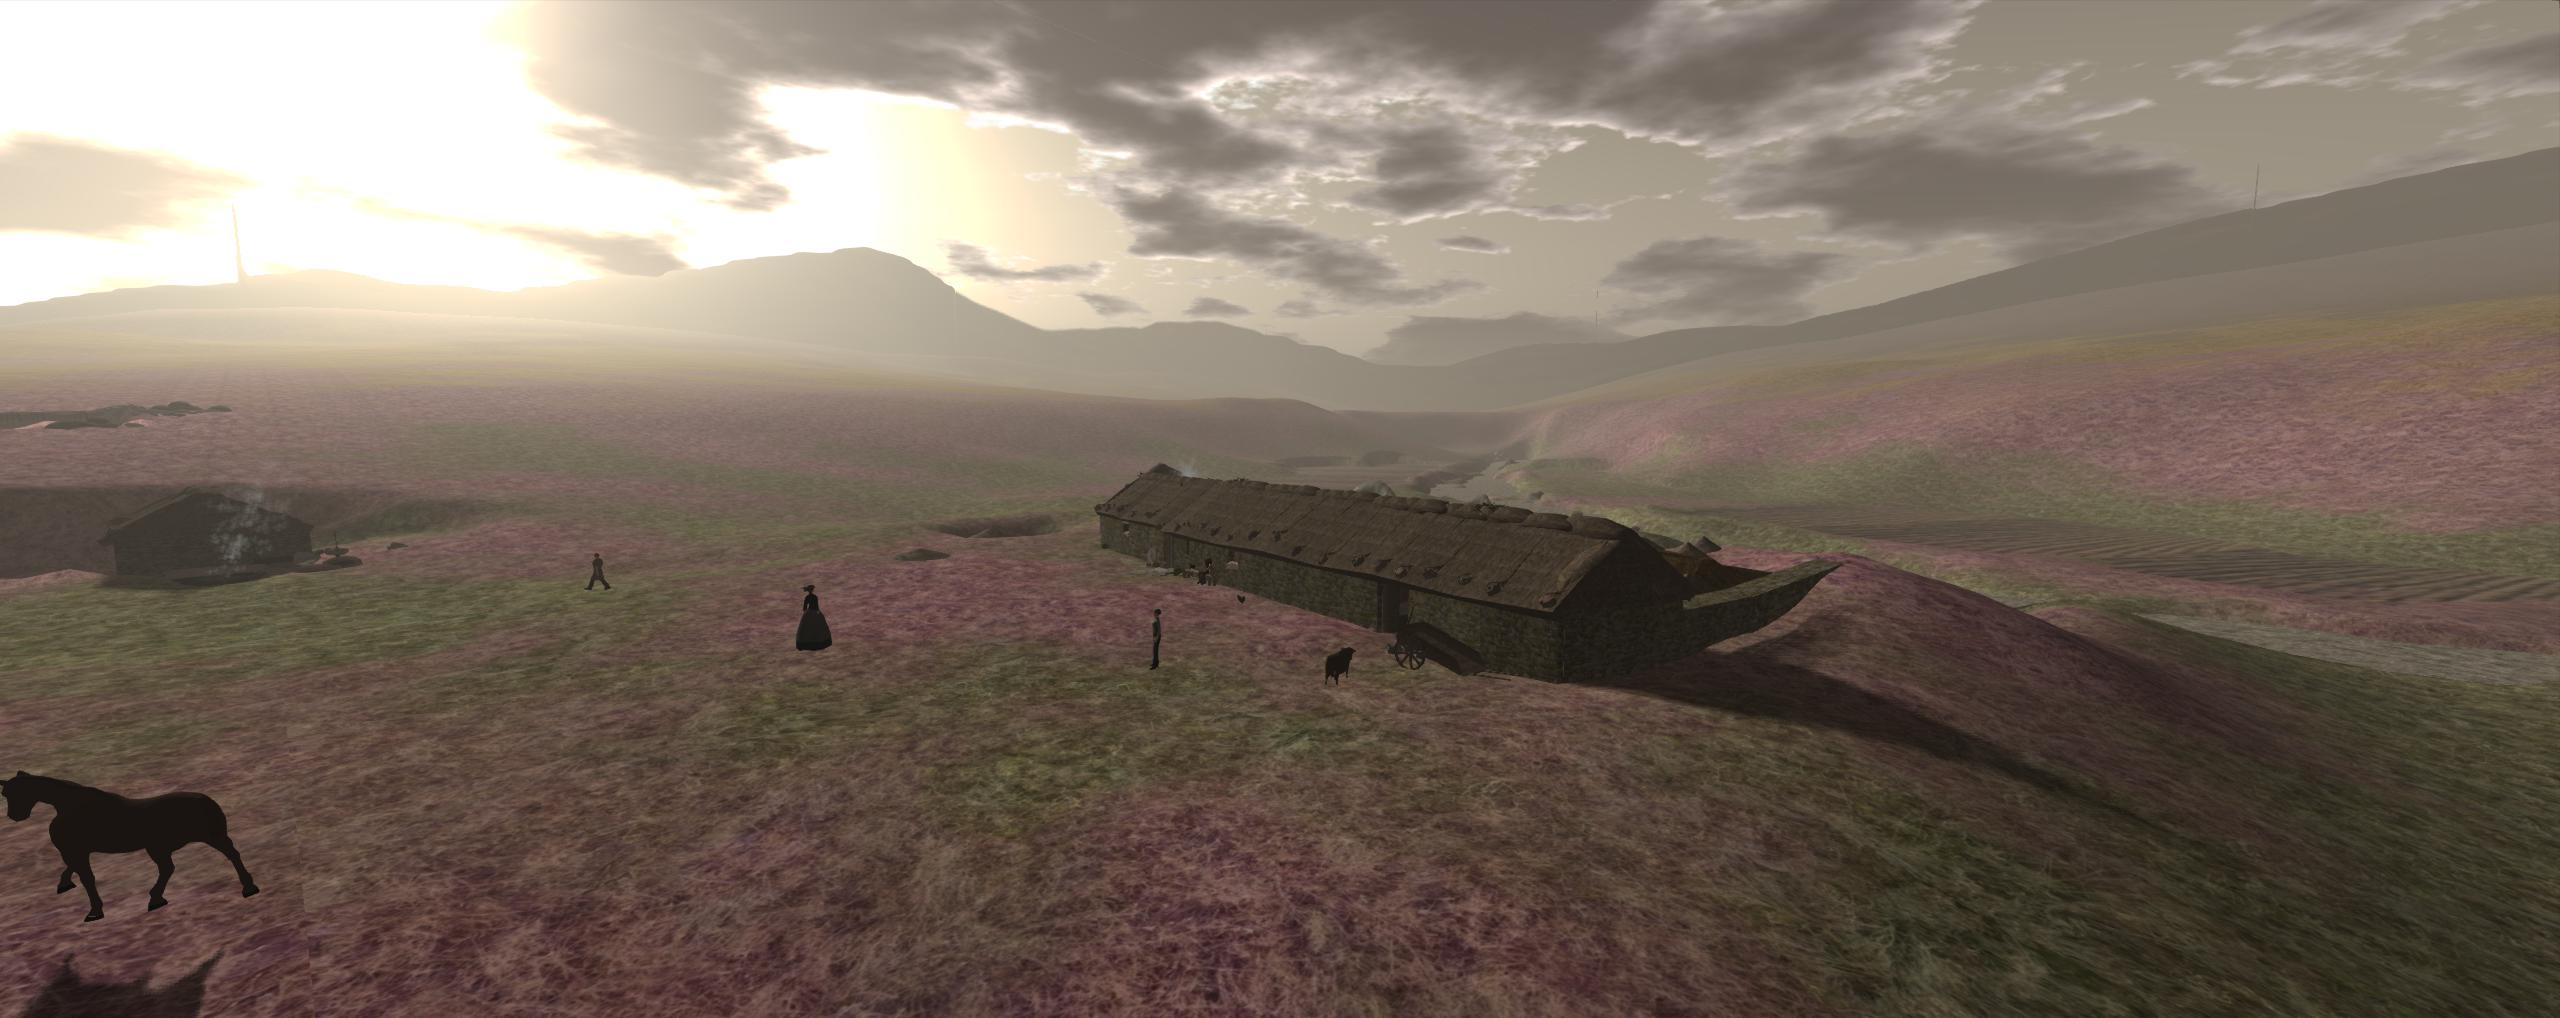
\includegraphics[width=\linewidth]{caen_township_outside.jpg}
  \caption{Caen Township reconstruction.}
  \label{caen_township_outside.jpg}
\end{figure}

\TwoFig{cathedral_npc_standing.png} {Virtual humans in cathedral reconstruction.} {cathedral_npc_standing.png}
       {cathedral_npc_talking.png} {Conversing with virtual humans in cathedral reconstruction.} {cathedral_npc_talking.png}

\pagebreak

These reconstructions were made using OpenSim, an open source implementation and extension of the Second Life server, which is compatible with the numerous forks of the Second Life client program. This architecture allows straightforward construction and dissemination of the models thanks to accessible modelling tools provided by the Second Life client itself and the client/server model of the platform that allows the reconstructions to be accessed in various deployment scenarios including temporary deployments within controlled network conditions as well as remotely via the Internet.

The reconstruction process involves the use of Geographic Information System (GIS) data from Ordnance Survey (OS) to accurately model the basic elevation of the ground. Where there is higher resolution elevation data, such as from Lidar laser surveying often employed on archaeological surveys, this is used to increase the accuracy of the resultant reconstruction. Where access to the site is possible and depending upon development surrounding the site prior to the date being reconstructed, 360\textdegree\ panoramic photographs are captured and used to create a backdrop for the reconstruction, allowing identifiable aspects of the surrounding environment to improve the experience of the reconstruction. Buildings/structures are then reconstructed upon the ground layer, using numerous sources as input; satellite views, archaeological surveys, contemporary accounts, views of the site itself (if evidence still exists), photographic evidence, etc. Domain experts are then consulted to iteratively improve the model, by commenting on aspects of the reconstruction to be altered in order to visualise different reconstructive hypotheses.

To date these reconstructions have been used to host workshops at 10 different schools throughout Scotland, including both primary and secondary institutions, where all requisite computing infrastructure was taken, assembled at the school, then disassembled and removed at the end of the day. Students were split into groups of 4-5, sharing a computer with screen, keyboard, mouse and Xbox controller (a control modality instantly recognised by most school students). Worksheets with tasks were used to structure their interaction with the reconstructions and guide the experiential learning process over 20-40 minute sessions (see figure \ref{linlithgow_children.jpg}). Similar workshops have also been performed in museums, using the same approach of temporary setups of computing hardware (see figure \ref{musa.jpg}). In addition to traditional computer screens, larger LCD television screens, still larger projection screens and Oculus Rift virtual reality HMDs have been used with this same content~(as seen in figure \ref{rift_exhibition.jpg}).

In addition to these temporary workshops, the reconstructions have also been used in permanently installed exhibits in museums and visitor centres, including the Virtual Time Travel Project (VTTP) which combines multi-head projection with Natural User Interaction (NUI) via Microsoft Kinect and has been installed at the Timespan Museum and Arts Centre in Helmsdale. VTTP allows visitors to explore the reconstruction of the Caen Township by using simple gestures instead of relying upon a keyboard, game controller or other tangible interface, and can be seen in figure \ref{VTTP_projection.png} and in a video available to view online\footnote{\url{https://vimeo.com/90968731}}.

\TwoFig{linlithgow_children.jpg} {School students learning with the Linlithgow Palace reconstruction.} {linlithgow_children.jpg}
       {rift_exhibition.jpg} {Presenting reconstructions via Oculus Rift.} {rift_exhibition.jpg}

\begin{figure}[h]
\centering
  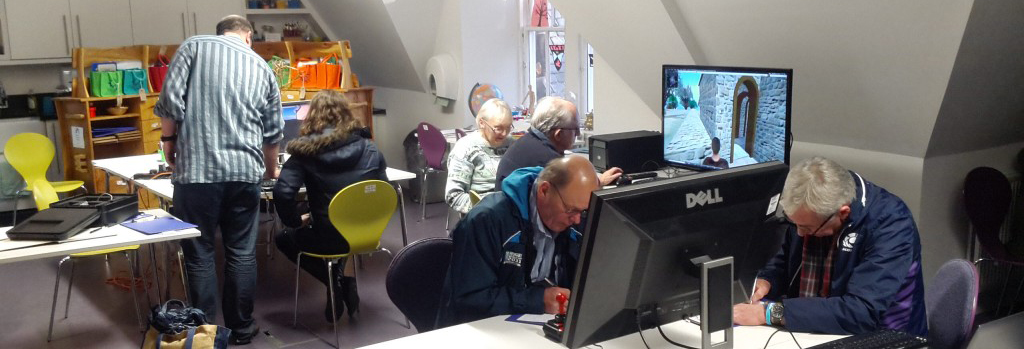
\includegraphics[width=\linewidth]{musa.jpg}
  \caption{Reconstructions used in a museum workshop.}
  \label{musa.jpg}
\end{figure}

\begin{figure}[h]
\centering
  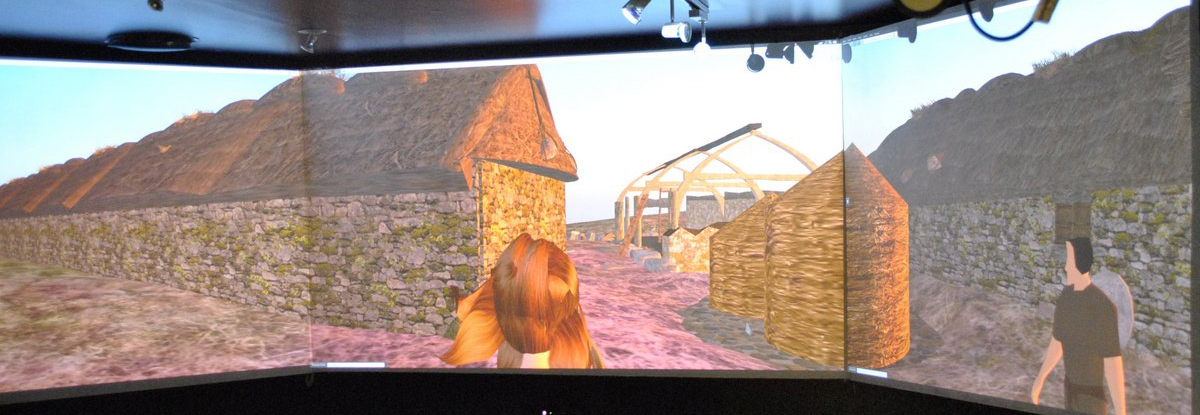
\includegraphics[width=\linewidth]{VTTP_projection.png}
  \caption{VTTP installation at Timespan Museum and Arts Centre.}
  \label{VTTP_projection.png}
\end{figure}

%=========================================================================================================

\subsection{Parallel Reality in Virtual Heritage}

\label{parallel-reality-in-virtual-heritage}

%Can we take the idea of sitsim, use it to leverage existing Second Life/OpenSim content, to produce a viable parallel reality experience?

Applications of alternate reality techniques within virtual heritage have thus far broadly fallen either into the category of augmented reality experienced at the site, or virtual reality experienced away from the site (in terms of space, time, or both), with sitsim representing one of the few exceptions. The dissemination of the OVW group's reconstructions has been no exception to this observation, falling into categories 10-12 of figures \ref{taxonomy_1.png} and \ref{taxonomy_2.png} by using complete virtual environments that are experienced with both spatial and temporal separation from the real sites that they represent.

Investigating the parallel reality concept by application to virtual heritage, possibly via the familiar modality of alternate reality interaction presented by a sitsim style interface, represents an opportunity to explore exciting new modalities of interaction that combine the complete virtual environments of categories 10-12 with the real time juxtaposition between real and virtual environments of augmented reality systems from category 13, in a real world use case situation. In terms of the four categories of the taxonomic space, parallel reality combines the high precision and interactivity of a virtual reality system (category 10) with two values of virtuality, as the user is provided the ability to alternately view the unmodified real environment (virtuality = 0) or the complete virtual environment (virtuality = 1). The automatism of such a system occupies a position between that of virtual reality and augmented reality; whilst the system requires a more involved development cycle than a purely virtual reality one, the relaxed requirements upon registrational accuracy of a parallel reality system compared to an augmented reality system promise higher automatism than a purely augmented reality system.

%=========================================================================================================

Although parallel reality as a concept is less critical of accurate registration than augmented reality, the accuracy of registration available particularly in terms of positional data represents a restriction upon the style of interaction possible with a parallel reality system, a point recognised by Liest\o l et al. during their sitsim experiments~\cite{Liestøl2012}. Considering a scale of increasing accuracy, three use cases for parallel reality within cultural heritage scenarios can be envisioned, with each representing increased interactivity in the terms of figure \ref{taxonomy_1.png}:

\begin{enumerate}
	\item Static viewpoints - Where the accuracy of the positioning system used by a parallel reality system is low, a style of interaction in which users move between predetermined points of interest at which they gain the ability to view the virtual environment from the equivalent vantage point is possible. In this scenario users are free to explore any vantages within the real environment, but are restricted to viewing the virtual environment from particular vantages chosen by curators for their particular importance, similar to indirect AR and the static AR experiences mentioned in section \ref{existing-virtual-heritage-applications}. The minimum distance between any pair of these viewpoints is dictated by the worst case accuracy of the positioning solution used by the parallel reality system.
	
	\item Freeform exploration - Where the accuracy of the positioning system is high enough to reliably differentiate a user's position between adjacent rooms/corridors, placing them on the correct side of walls and estimating their position within open areas, a style of interaction is possible wherein the user has the ability to view the virtual environment from the equivalent vantage point wherever they may be in the site. In this scenario users are free to explore and compare any vantages within both real and virtual environments, although direct comparison of small features/artefacts observed from less than several meters away may not be possible due to inaccuracy in the positioning solution.
	
	\item Freeform exploration with detailed comparison - Where extremely accurate positioning is available, a style of interaction that allows the user to not only explore and compare general aspects of the real and virtual environments from the equivalent vantage point but also to perform close comparisons of artefacts is possible. In this scenario not only can users freely compare between real and virtual when walking between different areas of a cultural heritage site, but they can more closely inspect any particular artefact and perhaps even interact with and affect them.
\end{enumerate}

%=========================================================================================================

\section{The Virtual Time Window}
\label{the-virtual-time-window}
The Virtual Time Window (VTW) was a preliminary investigation into the application of parallel reality to virtual heritage, that leveraged the OVW group's existing OpenSim reconstructions of cultural heritage sites in a handheld package that allows tandem exploration of both the real cultural heritage sites and their spatially equivalent virtual reconstructions. The challenge was not only to create a platform, leveraging the familiar modality of alternate reality interaction presented by existing sitsim implementations, that would allow investigation into the parallel reality concept in a virtual heritage scenario, but also to do so by making use of the OVW group's extensive catalogue of OpenSim based reconstructions. As discussed in section \ref{caseforpr} the ability of the parallel reality concept to make use of existing complete virtual models, without requiring a lengthy conversion phase of aspects of that content into an alternative format or framework, is one of its potential advantages. In the case of the OVW group's OpenSim content this approach also allows for potential interaction between on-site parallel reality visitors and remote participants interacting with the same models via a computer monitor, HMD, etc., thanks to OpenSim's distributed multi-user framework that leverages Internet connectivity.

VTW is presented as a tablet computer which is capable of tracking its position via GPS, its compass heading (yaw) via magnetometer (`electronic compass') and its pitch via accelerometer. Previous augmented reality and sitsim applications have proven the suitability of smartphones and tablets for mobile, position and orientation aware scenarios that present virtual objects within a cultural heritage context. These devices are entering ubiquity today, presenting a platform that can be quickly assimilated by most users.

The tablet employed by VTW runs a modified version of the Second Life client that accesses, via wifi, a virtual reconstruction of a cultural heritage site hosted by an OpenSim server. The Second Life client is controlled entirely by the tablet's position and orientation - the user does not manually control any aspect. The modality of interaction offered is similar to that of using a smartphone to take a photograph, but whereas the screen of the smartphone shows the real environment as it is, the screen of the VTW tablet shows the environment as it was in the past - a window to the past, or \textit{Virtual Time Window}. The user is free to explore the real cultural heritage site, observing it in its current state, whilst at any moment `looking through' VTW to see what a particular vantage looked like in the past. Figure \ref{vtw_high_level.png} provides a high level conceptual overview of the components of the platform.

\begin{figure}[h]
\centering
  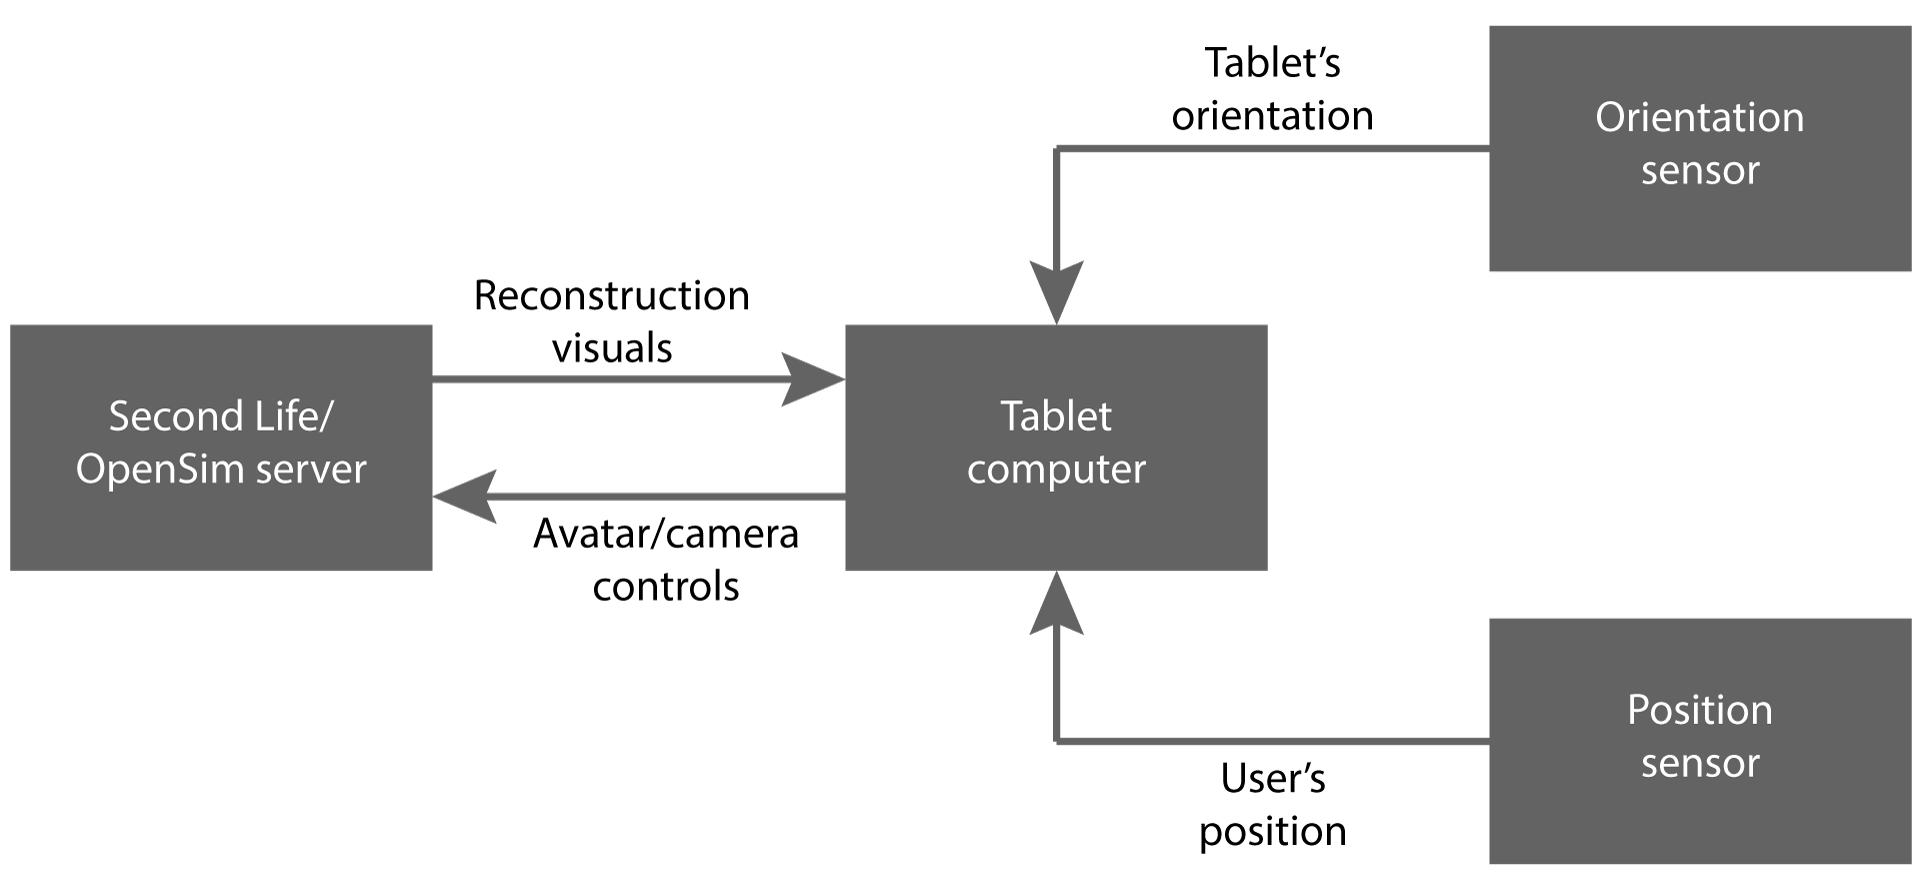
\includegraphics[width=.7\linewidth]{vtw_high_level.png}
  \caption{High level architecture of VTW parallel reality platform.}
  \label{vtw_high_level.png}
\end{figure}

From the perspective of transitioning between receiving stimuli from each environment, there is an obvious difference between VTW's tablet based approach compared to a HMD approach, as the latter effectively forces all percepts to emanate from one environment whilst the former allows percepts emanating from both environments to be perceived together with one in the periphery. Whilst this intuitively makes transitions easier to perform and creates less risk of a jarring Gestalt switch, it was also expected to limit immersion in the virtual environment as the sense of `looking in to' the virtual environment would always leave the user readily aware of the real environment surrounding it. In terms of the combined Milgram/Waterworth model, the displacement along the locus axis when the user switches their attention between their real environment and the virtual environment upon the tablet was expected to displace less toward the virtual reality extreme than shown in figure \ref{focus-locus-sensus-with-virtuality-continuum-with-transition}, which theorises transitions between real and virtual environments in which viewing the virtual entirely occludes the real (such as when using a HMD).

%Map showing spatial separation of Madras and cathedral?

%=========================================================================================================

\subsection{Second Life and Mobility}

\label{SecondLifeMobility}

\newcommand{\LumiyaFootnote}{\footnote{\url{https://play.google.com/store/apps/details?id=com.lumiyaviewer.lumiya&hl=en_GB}}}

\newcommand{\WindpadFootnote}{\footnote{\url{http://www.msi.com/product/windpad/WindPad-110W.html}}}

%=====================

At the time of the VTW project (Summer 2012) the only fully-featured Second Life clients available were for x86 platforms. Whilst the Android client Lumiya\LumiyaFootnote{} was available, it was in early stages of development and limited in its features and usability. This limited the choice of tablet for VTW to those few x86 models that had reached market, with the MSI WindPad 110W\WindpadFootnote{} presenting the most promising solution: a 10'' tablet sporting an AMD Brazos Z01 APU (combining a dual-core x86 CPU with a Radeon HD6250 GPU).

The Second Life client, intended for use on a desktop or laptop computer, provides provision for controlling the avatar's position and the camera orientation by keyboard, mouse and joystick. For the purposes of VTW, this position and orientation control had to be tied to the physical position and orientation of the tablet itself. To this end, it was necessary to make use of various sensors connected to the tablet (either internally, or externally) and to interface these with the Second Life client for it to use their collected data to appropriately control the avatar's position and camera orientation.

%\cite{willmott:largecomplex} occlusion culling etc., missing in Second Life/OpenSim

%Talk about history of Second Life/OpenSim in academia/research, including original cross reality research.

%The 3D virtual environment component of the Pangolin system was implemented using the Second Life/OpenSimulator (SL/OpenSim) platform, which provides a 3D social-oriented multi-user non-competitive virtual environment which focuses on the community, creation and commerce~\cite{Sevan2008} aspects of many users interacting within a shared space through the abstraction of avatars, rather than the competitive natures of games and the solitary environments commonly afforded by simulation and visualization platforms.

%The distributed client/server model of SL/OpenSim, wherein 3D content is stored on a grid of servers operated by a multitude of organizations and distributed to and navigated between by dispersed clients on demand when they enter a particular region rather than being pre-distributed as is the norm for games, simulations and visualizations, is analogous to the manner in which 2D social Web content is served from Web servers to client browsers and apps.

%This style of content delivery is necessary when considering the dynamic and ephemeral nature of consumer-generated media which constitutes the majority of the current 2D social Web and will make up the majority of expanding 3D social Web content.

%=========================================================================================================

\section{Orientation Control}

\label{OrientationControl}

\newcommand{\ArduinoFootnote}{\footnote{\url{http://www.arduino.cc/}}}

\newcommand{\MMAfootnote}{\footnote{\url{http://cache.freescale.com/files/sensors/doc/data_sheet/MMA8452Q.pdf}}}

\newcommand{\ADXLfootnote}{\footnote{\url{http://www.analog.com/static/imported-files/data_sheets/ADXL335.pdf}}}

\newcommand{\HMCfootnote}{\footnote{\url{http://www51.honeywell.com/aero/common/documents/myaerospacecatalog-documents/Defense_Brochures-documents/HMC5883L_3-Axis_Digital_Compass_IC.pdf}}}

\newcommand{\HMCtwoFootnote}{\footnote{\url{http://www51.honeywell.com/aero/common/documents/myaerospacecatalog-documents/Missiles-Munitions/HMC6343.pdf}}}

\newcommand{\HMCvccFootnote}{\footnote{The HMC6343 requires 2.7 to 3.6V input on VCC/VDD, this table showing connection to 5V assumes a HMC6343 breakout with appropriate step down.}}

\newcommand{\itwocFootnote}{\footnote{The HMC6343's I2C lines must be pulled up to 3.3V, this table shows connection to an Arduino Uno R3's I2C lines which are pulled up to 5V assuming a HMC6343 breakout with appropriate level shifters.}}

%http://www.nxp.com/documents/user_manual/UM10204.pdf

%=====================

In order to control Second Life's camera in the fashion required for VTW, sensor data were required for the orientation in which the user was holding the tablet. Specifically the tablet's yaw and pitch were needed; roll was considered less important as users were expected to hold the tablet roughly level with the horizon when looking `through' it.

VTW considers yaw in terms of magnetic compass bearing, as this provides a value that can be used to directly control the yaw of the virtual camera if the virtual reconstruction within OpenSim is correctly oriented to OpenSim's own compass. Magnetic compass bearings are sensed electronically via a 3-axis microelectromechanical (MEMS) magnetometer, which measures the strength of magnetic field along each of its 3 axes. By comparing the values of each axis to the known direction of the field lines of Earth's magnetic field, a compass bearing relative to the magnetometer's orientation can be calculated. Pitch is sensed using a 3-axis MEMS accelerometer, which measures force of acceleration along each of its 3 axes. In the case of static or slow moving applications, this acceleration is predominantly that caused by the Earth's gravitational pull and by comparing the values between each axis the direction of this acceleration (down toward the centre of the Earth) can be determined in relation to the orientation of the accelerometer itself and thus the accelerometer's own orientation (and that of the tablet it is attached to) can be deduced.

Due to the fact that the WindPad tablet does not feature a built-in magnetometer and its built-in accelerometer is little more than a rudimentary tilt sensor for differentiating between discrete cases of landscape and portrait orientation for screen rotation, it was necessary to interface external magnetometer and accelerometer sensors. The popular Arduino\ArduinoFootnote{} microcontroller platform was used for prototyping with several different sensor packages, including the MMA8452\MMAfootnote{}, the ADXL335\ADXLfootnote{} and the HMC5883L\HMCfootnote{}. The package eventually adopted for use with VTW from this prototyping stage was the HMC6343\HMCtwoFootnote{}, which combines a 3-axis MEMS magnetometer and 3-axis MEMs accelerometer into a single package sporting an I2C serial interface, along with algorithms to internally apply the accelerometer's readings to `tilt compensate' the magnetometer's readings. Figure \ref{arduino_wiring_hmc.png} provides a wiring diagram for connectivity of a HMC6343 to an Arduino Uno R3, with the pinout values provided by table \ref{HMC6343wiringtable}, while figure \ref{arduino_joystick_for_second_life_1.jpg} shows an assembled unit.

\begin{figure}[h]
\centering
  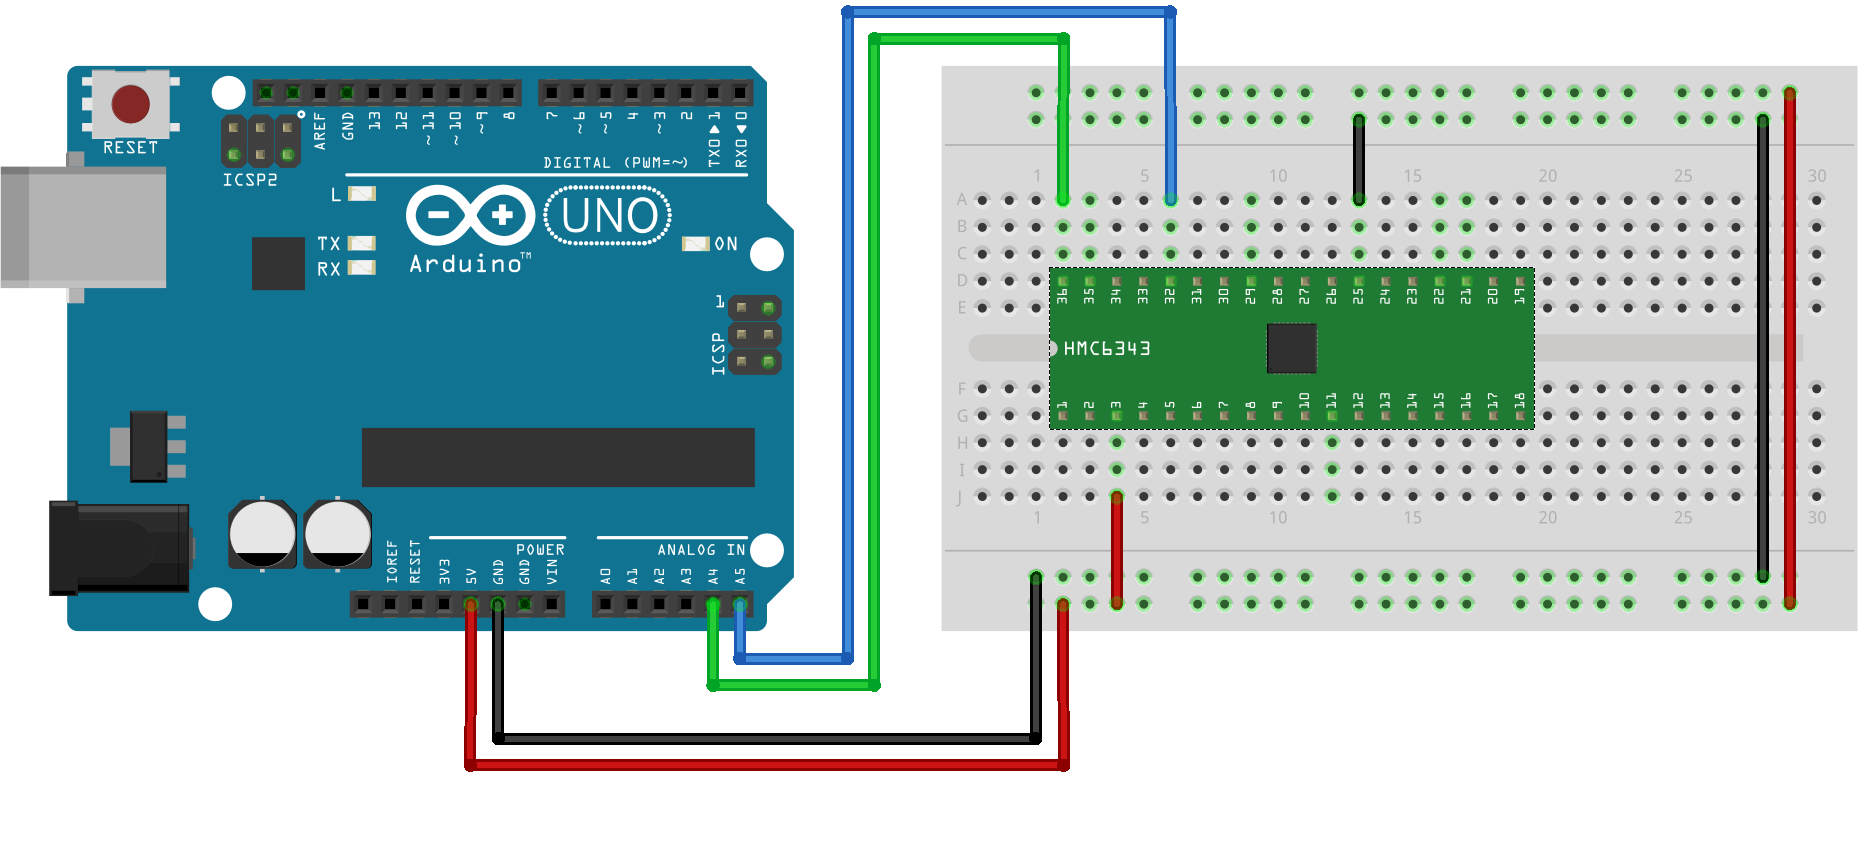
\includegraphics[width=\linewidth]{arduino_wiring_hmc.png}
  \caption{Wiring diagram for Arduino with HMC6343.}
  \label{arduino_wiring_hmc.png}
\end{figure}

%=====================

\begin{table}
\begin{center}
\begin{minipage}{.45\linewidth}
\begin{center}
\begin{tabularx}{\textwidth}{c *{2}{>{\centering\arraybackslash}X}}
\toprule
\textbf{HMC6343 pin} & \textbf{Arduino Uno R3 pin} \\
\midrule
VCC & 5V\HMCvccFootnote{} \\

GND & GND \\

SDA & A4\itwocFootnote{} \\

SCL & A5 \\
\bottomrule
\end{tabularx}
\end{center}
\end{minipage}
\end{center}
\caption{Pin designation for figure \ref{arduino_wiring_hmc.png}.}
\label{HMC6343wiringtable}
\end{table}

%=====================

\begin{figure}[h]
\centering
  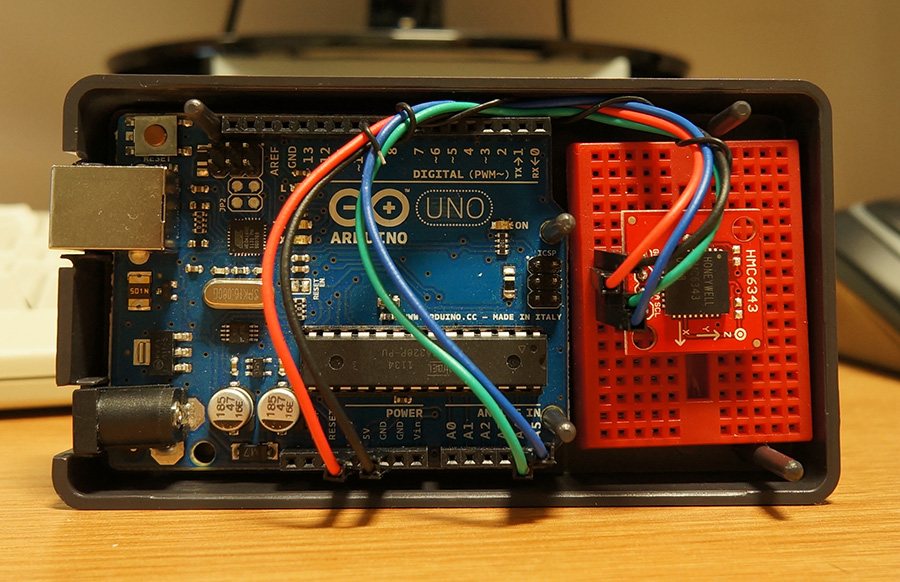
\includegraphics[width=.6\linewidth]{arduino_joystick_for_second_life_1.jpg}
  \caption{Assembled Arduino Uno R3 and HMC6343 package.}
  \label{arduino_joystick_for_second_life_1.jpg}
\end{figure}

Although the 10Hz update rate of the HMC6343 is much lower than those sported by the other packages, its combination of accelerometer and magnetometer into a single package ensured maximum accuracy: even a small discrepancy between the physical mounting of separate accelerometer and magnetometer packages would have been of noticeable detriment to the performance of the platform. The inclusion of tilt-compensation algorithms in the HMC6343 also allowed for easier and faster integration into VTW.

A magnetometer used independently is only capable of providing a meaningful compass bearing when held level. In the case of applications where a compass bearing is required of a device that is not maintained level, such as in the case of VTW, the non-level orientation of the device must be taken into account to offset the readings of the magnetometer and provide a correct compass bearing. The HMC6343's combination of magnetometer, accelerometer and algorithms provides a single package that internally performs this process, using the readings from its accelerometer to compensate the readings from its magnetometer and provide a meaningful compass bearing in non-level orientations.

Further requirements for obtaining accurate compass bearings from a MEMS magnetometer are to account for distortions to the magnetic field it senses and to compensate the bearings it reports for the amount of magnetic declination at the location and date whereupon it is used. Various materials that influence magnetic fields or produce their own magnetic field distort the Earth's magnetic field and this impacts the readings that a MEMS magnetometer collects. In the case of VTW, the primary sources of consideration were the electronics of the Arduino, tablet and associated wiring. Due to the nature of these sources and the fact that they were permanently situated and attached to the same frame of reference as the magnetometer, moving as it moves, the distortions could be mitigated using a hard iron offset approach\footnote{\url{http://www.freescale.com/files/sensors/doc/app_note/AN4246.pdf}}. Magnetic declination refers to the difference between `magnetic north' and geographic `true north' and varies depending upon world location and changes over time, so must be updated when the magnetometer is deployed to a different location or used at a subsequent date.

%***Reference for hard iron offset - here or later where we talk about the hex?

%=========================================================================================================

\subsection{Exploiting Second Life's Joystick Support}

\label{exploitJoystick}

\newcommand{\ArduinoJoystickVideoFootnote}{\footnote{\url{https://www.youtube.com/watch?v=-ddtmqoGNmg}}}

\newcommand{\atmegaFootnote}{\footnote{\url{http://www.atmel.com/devices/ATMEGA16U2.aspx}}}

\newcommand{\atmegaTFootnote}{\footnote{\url{http://www.atmel.com/devices/atmega328.aspx}}}

\newcommand{\arduinousbhidFootnote}{\footnote{\url{http://hunt.net.nz/users/darran/weblog/a3599/}}}

\newcommand{\lufaFootnote}{\footnote{\url{http://www.fourwalledcubicle.com/LUFA.php}}}

%=====================

As mentioned in section \ref{SecondLifeMobility} the Second Life client can be controlled only via mouse, keyboard and joystick. Using the HMC6343's compass bearing and yaw values therefore required one of two approaches:

\begin{enumerate}
	\item Encapsulating the compass bearing and yaw values into mouse, keyboard and/or joystick commands.
	\item Modifying the Second Life client to allow the compass bearing and yaw values to be used directly at a lower level of abstraction.
\end{enumerate}

Method 1 presented the advantage of maintaining compatibility with all Second Life clients, as all clients are forks of the same official client from Linden Lab and feature the same keyboard, mouse and joystick interfaces. However if the level of control attainable by re-purposing these interfaces for control from magnetometer and accelerometer data was not sufficient, method 2 would represent the only workable option.

Conceptually, all Arduino boards are programmed over an RS-232 serial connection. When the platform was first launched the Arduino boards themselves had a physical DE-9 serial connector with which to connect to a host computer's serial connector. But as serial connectors all but disappeared from modern computers the Arduino's serial connector was replaced in later revisions with a USB connector, as USB is now all but ubiquitous on today's computers. The move from a physical RS-232 connector to a USB connector required additional hardware upon the Arduino board to convert between RS-232 and USB, as the ATMega328\atmegaTFootnote{} microcontroller at the heart of the Arduino Uno R3 does not sport a USB interface itself. For this reason the current revision of the hardware, the Arduino Uno R3, sports an ATMega16U2\atmegaFootnote{} microcontroller that serves simply to convert communications between the two standards, RS-232 and USB.

With its stock firmware the Arduino's ATMega16U2 presents itself to the host computer as a USB-to-serial bridge, however this stock firmware can be replaced in order to change its behaviour. One alternative behaviour has it act as a USB Human Interface Device (HID) class controller, identifying itself to the host computer as one of myriad input devices - including joysticks. Using a USB HID class joystick firmware for the ATMega16U2\arduinousbhidFootnote{}, based upon the Lightweight USB Framework for AVRs (LUFA)\lufaFootnote{}, the Arduino can imitate a standard USB joystick, sending joystick commands to the host computer using the protocol of the USB specification.

%***How to flash the firmware

In this manner the Arduino could marshal the values obtained from the HMC6343 into standard USB HID joystick commands, allowing the Second Life client's stock joystick interface (see figure \ref{arduino_joystick_for_second_life_3.jpg}) to be used to control the camera orientation (and avatar movement) according to the physical orientation of the HMC6343. A simple example of this in action can be seen in a video available to view online\ArduinoJoystickVideoFootnote{}.

\begin{figure}[h]
\centering
  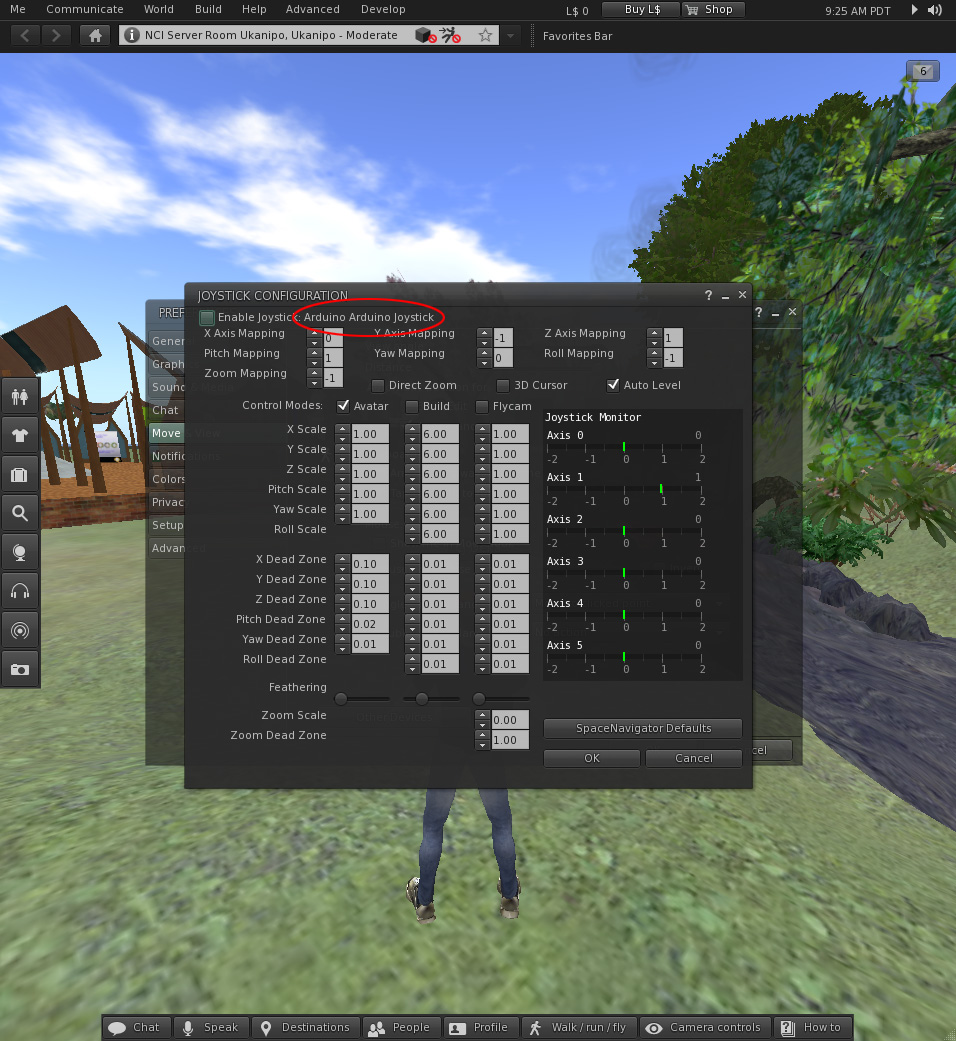
\includegraphics[width=.7\linewidth]{arduino_joystick_for_second_life_3.jpg}
  \caption{Configuration in Second Life client for Arduino and HMC6343 `joystick'.}
  \label{arduino_joystick_for_second_life_3.jpg}
\end{figure}

Unfortunately this experiment revealed that the precision attainable through this approach was not sufficient for the style of control and interaction required for VTW. Specifically the Second Life client's joystick interface seemed to apply smoothing/damping to the joystick inputs, preventing reliable rotations or movements of specific values: sending a joystick command to rotate the camera by $x$\textdegree\ followed by a second command to rotate the camera by $-x$\textdegree\ did not reliably return the camera to its original orientation from before the application of the first rotation. As the required interaction was to map the \textit{absolute} orientation of the tablet to the Second Life camera, this discrepancy (which cannot be disabled from the Second Life client's joystick configuration) rendered the approach unworkable.

%=========================================================================================================

\section{Position Control}
\label{second_life_position_control}

In order to control the position of the Second Life avatar, sensor data were required for the position of the user in the real world. VTW was intended for use at outdoor cultural heritage sites, where there are usually unobstructed views of the sky, so GPS represented the logical choice for tracking user position. GPS has been widely used as a localization technique within virtual heritage, particularly for augmented reality applications.

%***diagram showing this

In order for readings from a GPS receiver to be used to control the position of the Second Life avatar within a reconstruction, translations had to be performed between the coordinate system of GPS (latitude and longitude) and the coordinate system of Second Life (simple X,Y coordinates within 256 metre square `regions'). This was achieved by use of a single `anchor point' for which both the real world latitude and longitude and the corresponding virtual world X,Y coordinates were known. Calculating displacement within Second Life from these X,Y coordinates is achieved by applying the scale of the reconstruction to the displacement between the anchor point's latitude and longitude and the user's current position reported as latitude and longitude by a GPS receiver. This real world displacement is calculated using the haversine formula~\cite{VanBrummelen2012}, which is used to calculate the `great circle' (orthodromic) distance between two points on the surface of a sphere (such as the Earth, when simplified from its oblate spheroid shape). The central angle \text{$\left(\frac{d}{r}\right)$} between the two points is given by:

\begin{equation}
\label{haversine1}
\text{haversin}\left(\frac{d}{r}\right) = \text{haversin}(\phi_{2}-\phi_{1})+\cos(\phi_{1})\cos(\phi_{2})\text{haversin}(\lambda_{2}-\lambda_{1})
\end{equation}

where:

\begin{itemize}
	\item \text{haversin} is the haversine function:
		\begin{equation}
		\label{harsine2}
			\text{haversin}(\theta) = \sin^{2}\left( \frac{\theta}{2}\right) = \frac{1-\cos(\theta)}{2}
		\end{equation}
	\item $d$ is the distance between the two points along a great circle of the sphere.
	\item $r$ is the radius of the sphere.
	\item \text{$\phi_{1},\phi_{2}$} are the latitudes of point 1 and point 2.
	\item \text{$\lambda_{1},\lambda_{2}$} are the longitudes of point 1 and point 2.
\end{itemize}

The equation can be solved for the distance $d$ by applying the inverse haversine function or through application of arcsine:

\begin{equation}
	\label{haversine3}
	d = r\;\text{haversin}^{-1}\left( h \right) = 2r \arcsin \left( \sqrt{h} \right)
\end{equation}

where $h$ is $\text{haversin}\left( \frac{d}{r} \right)$:

\begin{align}
d & = 2r \arcsin\left( \sqrt{\text{haversin} \left( \phi_{2} - \phi_{1} \right) + \cos \left( \phi_{1} \right) \cos  \left( \phi_{2} \right) \text{haversin} \left( \lambda_{2} - \lambda_{1} \right) } \right) \nonumber \\ 
& = 2r \arcsin\left( \sqrt{\sin^{2} \left( \frac{\phi_{2} - \phi_{1}}{2}\right) + \cos\left( \phi_{1} \right) \cos\left( \phi_{2} \right) \sin^{2} \left( \frac{\lambda_{2} - \lambda_{1}}{2} \right) } \right)
\end{align}

The prerequisites for this approach were that the Second Life model be aligned correctly to the Second Life compass as the real location is aligned to real compass bearings (also required for orientation control, as mentioned in the previous section), a single `anchor point' for which both the real world latitude and longitude and the corresponding virtual world X and Y coordinates are known, and that the reconstruction adhered to a known consistent scale.

Figure \ref{haversine_example.png} illustrates the approach. In the real world on the left, we know the latitude and longitude of the anchor point as well as the latitude and longitude of the user's current position as reported by the GPS receiver. In the virtual world on the right, we know the X,Y coordinates that are equivalent to the latitude and longitude of the anchor point and we must calculate the X,Y coordinates that are equivalent to the user's current position as reported by the GPS receiver.

\begin{figure}[h]
\centering
  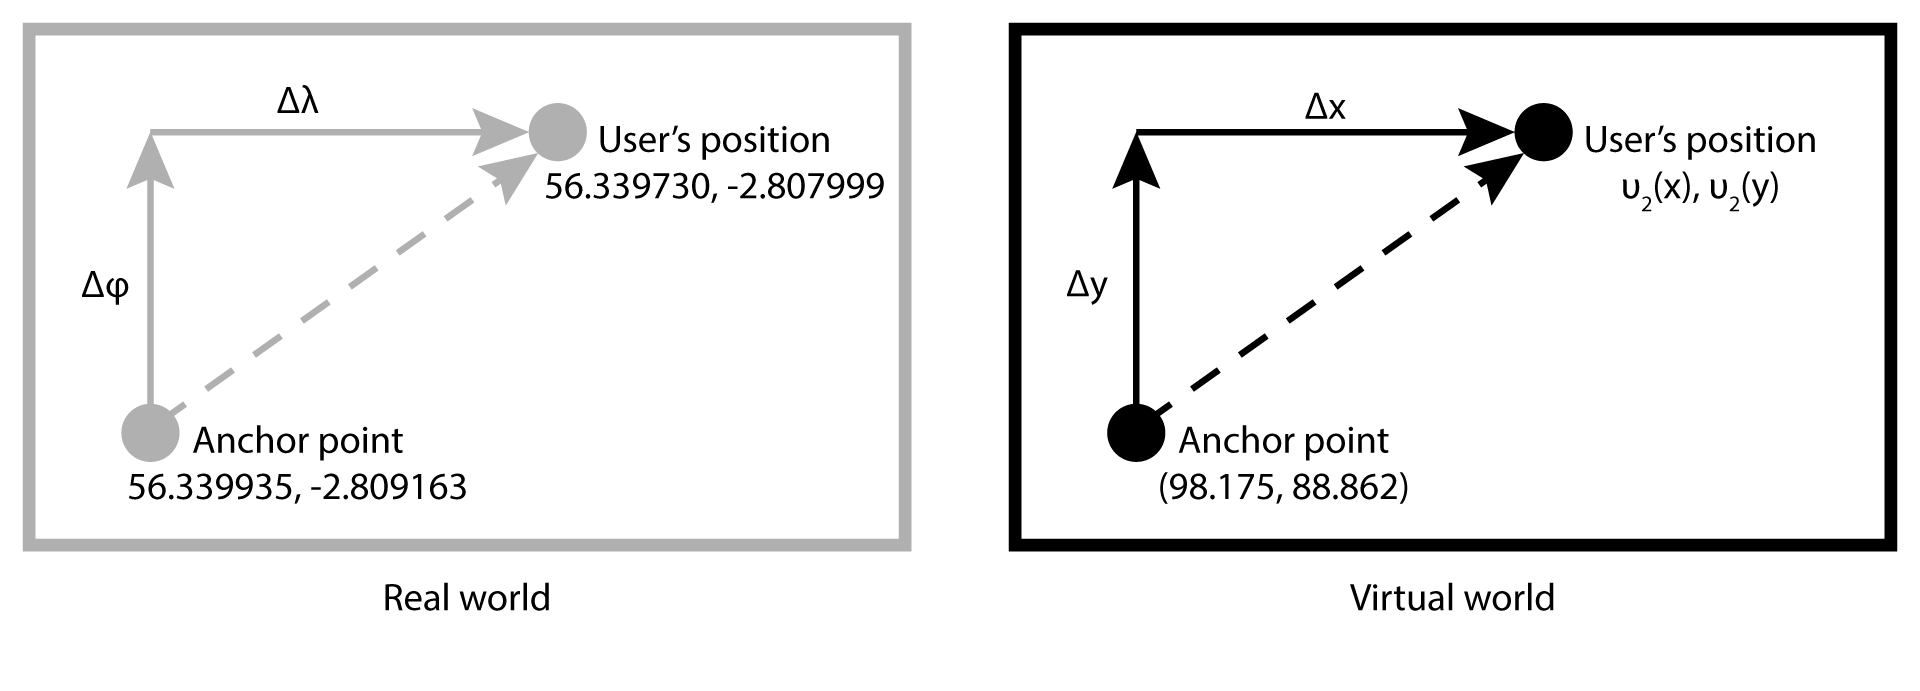
\includegraphics[width=\linewidth]{haversine_example.png}
  \caption{Visualisation of how haversine is applied to mimic real world movement in a virtual environment.}
  \label{haversine_example.png}
\end{figure}

The difference in longitude between the anchor point and the user's position, $\Delta\lambda$, is given by:

\begin{equation}
2r \arcsin\left( \sqrt{\sin^{2} \left( \frac{\lambda_{2} - \lambda_{1}}{2} \right) } \right)
\end{equation}

While the difference in latitude between the anchor point and the user's position, $\Delta\phi$, is given by:

\begin{equation}
2r \arcsin\left( \sqrt{\sin^{2} \left( \frac{\phi_{2} - \phi_{1}}{2}\right)} \right)
\end{equation}

Applying the scale of the reconstruction to these values gives $\Delta$x and $\Delta$y, which are then added to or subtracted from the X,Y coordinates of the anchor point to give the coordinates of the user's position, $\upsilon_{2}(x),\upsilon_{2}(y)$.

%Using the haversine formula the great-circle (or orthodromic) distance between the latitude of the anchor point and the latitude of the new GPS reading is calculated, then applying the scale of the model results in the equivalent distance in OpenSim metrics between the Y coordinate of the anchor point and the Y coordinate of the position corresponding to the new GPS reading. Repeating the same calculations with the longitude of the new GPS reading provides the distance between the X coordinate of the anchor point and the X coordinate of the position corresponding to the new GPS reading. Adding or subtracting these distances as appropriate to the OpenSim coordinates of the anchor point provides the OpenSim coordinates that correspond to the new GPS reading, to which the avatar is then instructed to move.

%The anchor point is specified using global coordinates, not local coordinates. This allows navigation to operate across region boundaries and within mega regions (it is not limited to a single 256x256 meter OpenSim region) and there are no restrictions for the placement of the OpenSim component of the anchor point (it can be anywhere in any region, movement of the avatar can be in any direction from it (positive and negative), it does not have to be at the center of the model or even in a region that the model occupies).

%Calculating a global coordinate is simply a case of multiplying the position of the region by 256 and then adding the local coordinate. For example, for an anchor at local coordinate $(127,203,23)$ within a region that is at $(1020,1042)$ the global X coordinate is calculated as $(1020 * 256) + 127 = 261247$ and the global Y coordinate as $(1043 * 256) + 203 = 267211$. Elevation (Z) is ignored due to a combination of the relatively low accuracy of these data attainable via GPS (when compared to the longitudinal/latitudinal accuracy) and as the case study explored involved users navigating outdoor ruins remaining at ground level.

%=========================================================================================================

\subsection{GPS Receivers}

\newcommand{\azurewaveFootnote}{\footnote{\url{http://www.azurewave.com/product_GPS-M19_1.asp}}}

\newcommand{\habFootnote}{\footnote{\url{http://ukhas.org.uk/}}}

\newcommand{\ubloxFootnote}{\footnote{\url{https://u-blox.com/en/gps-modules/pvt-modules/previous-generations/max-6.html}}}

\newcommand{\sarantelFootnote}{\footnote{\url{http://www.sarantel.com/sl1200_(33).html}}}

\newcommand{\MAXvccFootnote}{\footnote{The MAX-6 requires 2.5 to 3.6V input on VCC, this table showing connection to 5V assumes a MAX-6 breakout with appropriate step down.}}

\newcommand{\MAXserialFootnote}{\footnote{The data pins of the MAX-6 need to be pulled up to between 0.7 to 1.0 of the supply to VCC, so a breakout with appropriate level shifters is required for connection directly to an Ardunio Uno R3's 5V digital pins.}}

\newcommand{\softwareserialFootnote}{\footnote{\url{http://arduino.cc/en/Reference/SoftwareSerial}}}

\newcommand{\maxProtocolFootnote}{\footnote{\url{https://u-blox.com/images/downloads/Product_Docs/u-blox6_ReceiverDescriptionProtocolSpec_(GPS.G6-SW-10018).pdf}}}

\newcommand{\tinygpsFootnote}{\footnote{\url{http://arduiniana.org/libraries/tinygps/}}}

%=====================

The WindPad features an internal AzureWave GPS-M16 GPS receiver\azurewaveFootnote{}, however poor API provision and meagre documentation required the adoption of an alternative receiver. As an Arduino was already being used to provide orientation data from accelerometer and magnetometer, integrating the GPS receiver into this package such that all orientation and position data came from a single interface was prudent. After receiving input and advice from the UK High Altitude Society, \textit{``a loose collection of people who are interested in launching unmanned high altitude balloons into near space''}\habFootnote{} who make extensive use of GPS receivers for tracking their launches, the u-blox MAX-6\ubloxFootnote{} GPS receiver outfitted with a Sarantel SL-1202\sarantelFootnote{} passive antenna was chosen to provide position data for the VTW platform. The MAX-6 is of higher operational specification than the GPS-M16 and supports Satellite Based Augmentation Systems (SBAS), which improves the accuracy of location data by applying additional correction data received from networks of satellites and ground-based transmitters separate to those of the GPS satellites. These networks include the European Geostationary Navigation Overlay Service (EGNOS) that covers the UK where the VTW platform was developed and evaluated.

Figure \ref{arduino_wiring_hmc_ublox.png} provides a wiring diagram for connectivity of a u-blox MAX-6 to an Arduino Uno R3, along with the HMC6343 from section \ref{OrientationControl}, with the pinout values provided by tables \ref{HMC6343_MAX6_wiringtable_HMC6343} and \ref{HMC6343_MAX6_wiringtable_MAX6}. The LED and 220$\Omega$ resistor on digital pin 12 is used for diagnostic output. The wiring shown here is for a MAX-6 breakout without I2C connectivity, instead using Arduino's SoftwareSerial\softwareserialFootnote{} library. Figure \ref{arduino_hmc6343_u-blox_MAX-6.jpg} shows the assembled unit, comprising an Arduino Uno R3, prototyping shield, HMC6343 and MAX-6, while figure \ref{pangolin_tablet_back.jpg} shows this package attached to the back of the WindPad with the single required USB cable connecting the two.

\begin{figure}[h]
\centering
  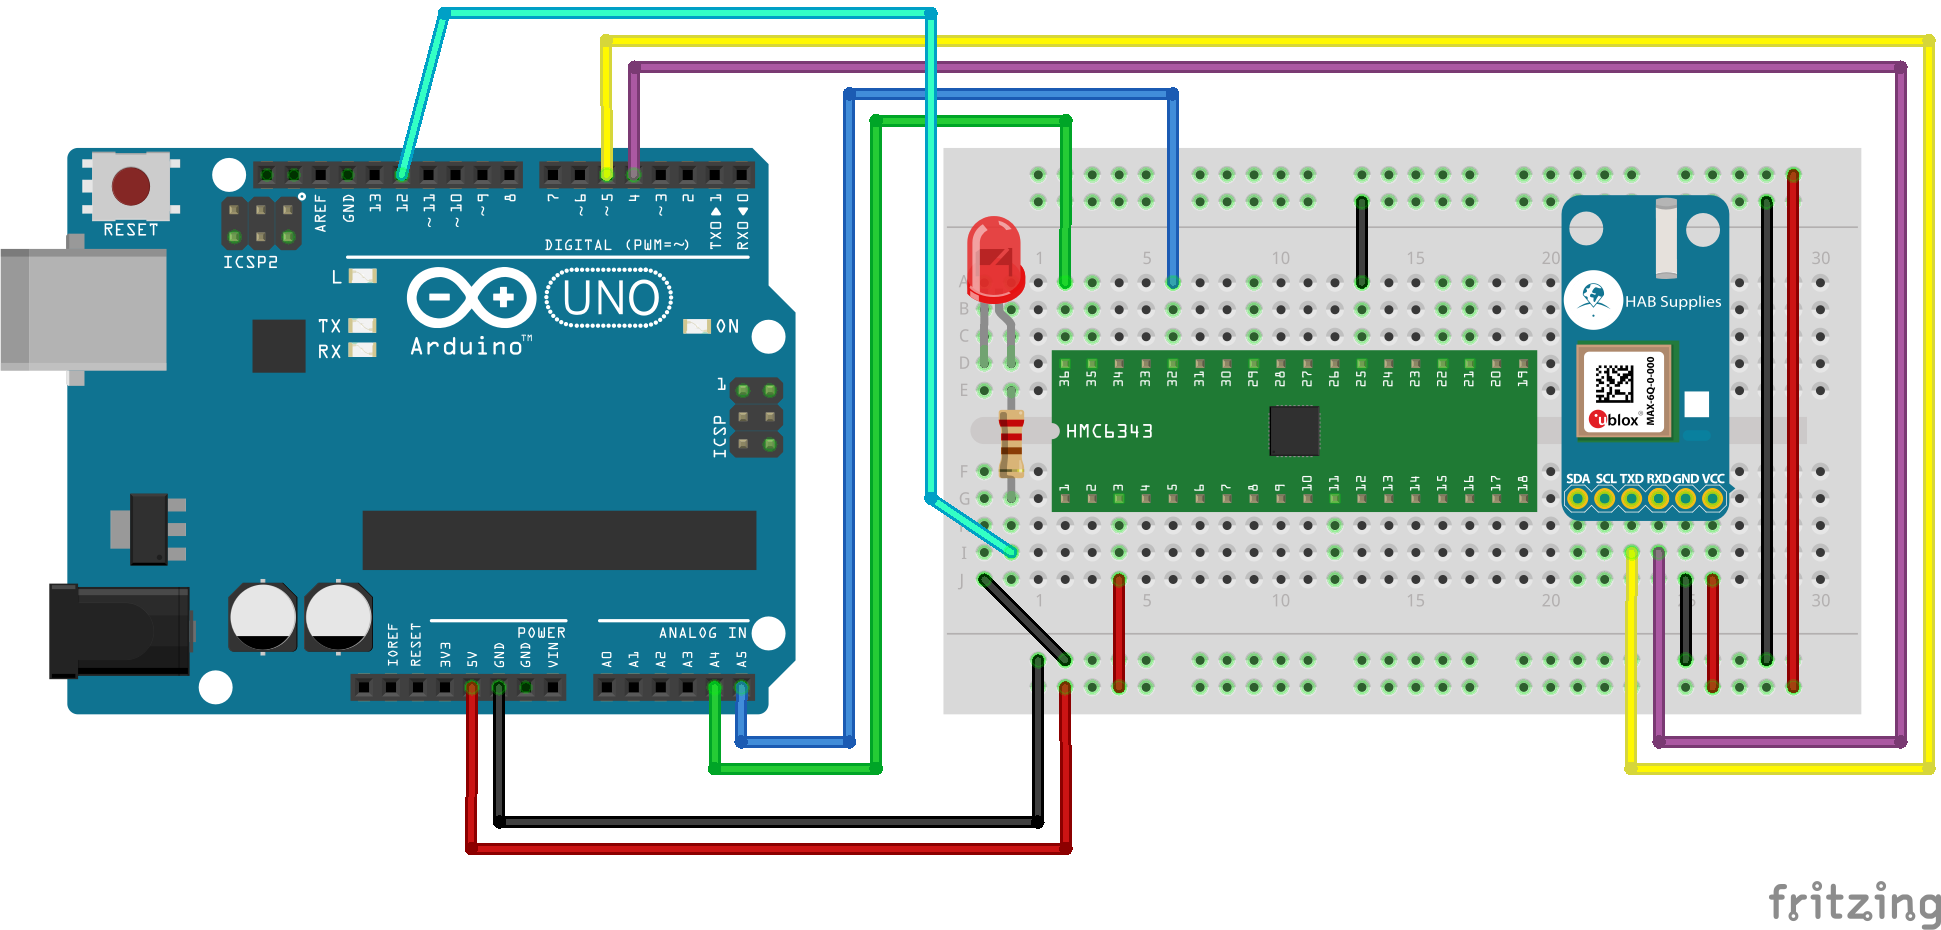
\includegraphics[width=\linewidth]{arduino_wiring_hmc_ublox.png}
  \caption{Wiring diagram for Arduino with HMC6343 and u-blox MAX-6.}
  \label{arduino_wiring_hmc_ublox.png}
\end{figure}

\begin{table}
\begin{center}
\begin{minipage}[t]{.45\linewidth}
\begin{center}
\begin{tabularx}{\textwidth}{c *{2}{>{\centering\arraybackslash}X}}
\toprule
\textbf{HMC6343 pin} & \textbf{Arduino Uno R3 pin} \\
\midrule
VCC & 5V\HMCvccFootnote{} \\

GND & GND \\

SDA & A4\itwocFootnote{} \\

SCL & A5 \\
\bottomrule
\end{tabularx}
\caption{Pin designation for figure \ref{arduino_wiring_hmc_ublox.png} (HMC6343).}
\label{HMC6343_MAX6_wiringtable_HMC6343}
\end{center}
\end{minipage}
%
\begin{minipage}[t]{.02\linewidth}
\hfill%
\end{minipage}
%
\begin{minipage}[t]{.45\linewidth}
\begin{center}
\begin{tabularx}{\textwidth}{c *{2}{>{\centering\arraybackslash}X}}
\toprule
\textbf{MAX-6 pin} & \textbf{Arduino Uno R3 pin} \\
\midrule
VCC & 5V\MAXvccFootnote{} \\

GND & GND \\

RXD & D4 \MAXserialFootnote{}\\

TXD & D5 \\
\bottomrule
\end{tabularx}
\caption{Pin designation for figure \ref{arduino_wiring_hmc_ublox.png} (MAX-6).}
\label{HMC6343_MAX6_wiringtable_MAX6}
\end{center}
\end{minipage}
\end{center}
\end{table}

\TwoFig{arduino_hmc6343_u-blox_MAX-6.jpg} {Assembled Arduino/sensor package used by VTW.} {arduino_hmc6343_u-blox_MAX-6.jpg}
       {pangolin_tablet_back.jpg} {Arduino/sensor package attached to tablet used by VTW.} {pangolin_tablet_back.jpg}
       
%=========================================================================================================

The MAX-6 was configured as follows:

\begin{enumerate}
	\item Dynamic Platform Model set to Pedestrian.
	\item SBAS via EGNOS enabled.
	\item GPGLL/GPGSA/GPGSV/GPVTG messages disabled.
	\item GPRMC/GPGGA messages enabled.
\end{enumerate}

The Dynamic Platform Models adjust how the onboard navigation engine processes the readings that the receiver produces and by choosing the correct model for the receiver's application the accuracy of position output is increased. As VTW is an application in which the user walks about an outdoor cultural heritage site, the pedestrian model is most suitable. SBAS is enabled for the EGNOS, which is available at cultural heritage sites within Scotland, in order to improve the accuracy of the position output.

The output of the receiver is in the form of messages in the NMEA 0183 protocol from the National Marine Electronics Association\footnote{\url{https://www.nmea.org/content/nmea_standards/nmea_0183_v_410.asp}}. By default the MAX-6 sends many more message types than are required for VTW and as the Arduino's processing power is limited the superfluous messages were disabled. The GPRMC message format contains the recommended minimum amount of information for transit applications, including time, latitude and longitude, which covers all of the position information required by VTW.

These configurations were effected by sending the MAX-6 commands encoded in the UBX protocol as arrays of hex values, which the Arduino is capable of doing at power on. For example, setting the Dynamic Platform Model to Pedestrian is performed with the code in figure \ref{arduinoMAX6hex}, where \path{sendUBX} is a function that writes to the MAX-6 using SoftwareSerial.

\begin{figure}[h]
\begin{lstlisting}[language=C, numbers=left, numberstyle=\small, stepnumber=1, frame=single, breaklines=true, backgroundcolor=\color{codebackground}, showstringspaces=false]
uint8_t CFG_NAV5[] = {0xB5, 0x62, 0x06, 0x24, 0x24, 0x00, 0xFF, 0xFF,
                      0x03, 0x03, 0x00, 0x00, 0x00, 0x00, 0x10, 0x27,
                      0x00, 0x00, 0x05, 0x00, 0xFA, 0x00, 0xFA, 0x00,
                      0x64, 0x00, 0x2C, 0x01, 0x32, 0x3C, 0x00, 0x00,
                      0x00, 0x00, 0x00, 0x00, 0x00, 0x00, 0x00, 0x00,
                      0x00, 0x00, 0x00, 0x00};
calculateUBXChecksum(CFG_NAV5, (sizeof(CFG_NAV5)/sizeof(uint8_t)));

while (!success)
{
  sendUBX(CFG_NAV5, (sizeof(CFG_NAV5)/sizeof(uint8_t)));
  success = getUBX_ACK(CFG_NAV5);
}
success = 0;
\end{lstlisting}
\caption{Setting MAX-6 Dynamic Platform Model to Pedestrian in an Arduino sketch.}
\label{arduinoMAX6hex}
\end{figure}

These hex arrays can be generated by hand from the UBX protocol specification\maxProtocolFootnote{}, or by connecting the MAX-6 directly to a host computer (such as by using an Arduino as a Universal Asynchronous Receiver/Transmitter (UART) by connecting the MAX-6 to digital pins 0 and 1) and using the u-blox u-center\footnote{\url{https://u-blox.com/en/evaluation-tools-a-software/u-center/u-center.html}} software, copying the resultant config as hex messages from the relevant console window.

NMEA messages from the MAX-6 are processed on the Arduino using the TinyGPS library\tinygpsFootnote{}, extracting the latitude and longitude values before combining them with magnetic compass bearing (yaw) and pitch values from the HMC6343 and sending these to the tablet via the Arduino's USB connectivity.

%=========================================================================================================

\subsection{OpenSim Region Module}

\label{regionModule}

\newcommand{\RegionModuleFootnote}{\footnote{\url{http://opensimulator.org/wiki/IRegionModule}}}

\newcommand{\RegionModuleCodeFootnote}{\footnote{\url{https://bitbucket.org/cj_davies/sharedregionmodulegpsavatar}}}

%=====================

One of the extensions that the OpenSim server provides over the Second Life server that it emulates is extensibility via Region Modules.

\begin{quotation}
	\textit{``Region modules are .net/mono DLLs. During initialization of the simulator, the OpenSimulator bin directory (bin/) and the scriptengines (bin/ScriptEngines) directory are scanned for DLLs, in an attempt to load region modules stored there. Region modules execute within the heart of the simulator and have access to all its facilities. Typically, region modules register for a number of events, e.g. chat messages, user logins, texture transfers, and take what ever steps are appropriate for the purposes of the module.''}\RegionModuleFootnote{}
\end{quotation}

Region modules allow for more complex and powerful extensions written in \texttt{C\#} to be developed, external to the OpenSim platform, than would otherwise be possible via Second Life's internal Linden Scripting Language (LSL). Similar to how the Second Life client's joystick interface represented an opportunity to implement the orientation control of VTW without relying upon a bespoke, modified client, an OpenSim Region Module represented a possibility to implement the position control required by VTW without similar reliance upon a bespoke client.

An excerpt from the implementation of the VTW position control as a region module is included as figure \ref{RegionModuleCode1} (the full region module code is available online\RegionModuleCodeFootnote{}). This shows the use of haversine, implemented using the \texttt{atan2()} function, calculating the displacement in real world latitude between the anchor point and the new GPS reading (lines 5-8), applying the scale of the reconstruction to this displacement (lines 10-14) and then applying this scaled displacement to the virtual world Y coordinate of the anchor (lines 16-24). This process is then repeated for the longitude/X coordinate and the avatar is then be moved to the position within the OpenSim reconstruction that is equivalent to the user's new real world position. Unlike using the joystick interface to effect camera control without modifying the Second Life client, this region module approach to position control successfully produced usable results.

\begin{figure}[h]
\begin{lstlisting}[language=Java, numbers=left, numberstyle=\small, stepnumber=1, frame=single, breaklines=true, backgroundcolor=\color{codebackground}, showstringspaces=false]
private Vector3 LatitudeLongitudeToRegionCoordinate(double newLat, double newLong, double anchorLat, double anchorLong, Vector3 anchorVector, double scale) {

    double d, a, c, X, Y;

    //calculate the difference in y (latitude) between the anchor & the new reading
    d = Math.Abs(ToRadians(newLat - anchorLat));
    a = Math.Sin(d / 2) * Math.Sin(d / 2);
    c = 2 * Math.Atan2(Math.Sqrt(a), Math.Sqrt(1 - a));

    //mean radius of the Earth is 6371km (6371000m)
    d = 6371000 * c;

    //apply scale
    d *= scale;

    //sum appropriately from the anchor
    if (newLat > anchorLat) {
        mlog.DebugFormat("[GPSAvatarModule]: LatitudeLongitudeToRegionCoordinate() - (Y) newLat > anchorLat.");
        Y = (anchorVector.Y + d);
    }
    else {
        mlog.DebugFormat("[GPSAvatarModule]: LatitudeLongitudeToRegionCoordinate() - (Y) newLat < anchorLat.");
        Y = (anchorVector.Y - d);
    }
\end{lstlisting}
\caption{Excerpt of OpenSim Region Module for avatar movement via GPS.}
\label{RegionModuleCode1}
\end{figure}

%=========================================================================================================

%\clearpage

%=========================================================================================================

\section{Modifying Second Life for Orientation and Position Control}

Due to the Second Life client's existing control interfaces not allowing enough control over camera orientation for VTW's requirements (section \ref{exploitJoystick}), it was necessary to modify the client's codebase to produce a bespoke client allowing complete control over orientation by magnetometer and accelerometer input. Although sufficient position control was obtained via an OpenSim region module (section \ref{regionModule}) it was deemed prudent to also encapsulate position control into the modified client. This not only allowed for finer grain control, but also removed the dependency upon the virtual reconstruction being hosted upon an OpenSim server; Second Life's own servers do not support extension via Region Modules. Thus the Second Life client was modified with the addition of the ability to:

\begin{itemize}
	\item Connect to a serial device for input/output.
	\item Control movement of the avatar according to input from this serial device.
	\item Control the camera according to input from this serial device.
\end{itemize}

%=========================================================================================================

\subsection{Overview of Second Life Client Modifications}

\newcommand{\asioFootnote}{\footnote{\url{http://www.boost.org/doc/libs/1_57_0/doc/html/boost_asio.html}}}

\newcommand{\boostFootnote}{\footnote{\url{http://www.boost.org/}}}

\newcommand{\fedetftFootnote}{\footnote{\url{http://www.webalice.it/fede.tft/serial_port/serial_port.html}}}

\newcommand{\regionmodulelimitationFootnote}{\footnote{This is not due to any limitation on the part of OpenSim, but simply due to the Second Life client modifications being pursued further than the OpenSim region module.}}

\newcommand{\megaregionFootnote}{\footnote{\url{http://opensimulator.org/wiki/Setting_Up_Mega-Regions}}}

%=====================

%Replaced the Linden Boost binary with that built by LightDrake

The Second Life client is written predominantly in \texttt{C++} so the Asio library\asioFootnote{} from the popular Boost project\boostFootnote{} was used to imbue it with serial connectivity, allowing it to receive messages from the Arduino in an asynchronous non-blocking fashion. The fundamental buffered asynchronous serial handling was implemented using Terraneo Federico's \path{AsyncSerial} class\fedetftFootnote{} which is included in the client codebase as \path{/indra/newview/AsyncSerial}. The majority of the functionality added to the client was then implemented within \path{/indra/newview/LLViewerSerialMovement}. The core executable of the viewer \path{/indra/newview/LLAppViewer} obtains an instance of \path{LLViewerSerialMovement} and calls \path{LLViewerSerialMovement::update()} upon each iteration of the client's main update loop \path{LLAppViewer::mainLoop()}. These modifications are visualised by figure \ref{second_life_structure.png} and the modified client codebase is available in full online\footnote{\url{https://bitbucket.org/cj_davies/viewer-release-serial-io}}.

\begin{figure}[h]
\centering
  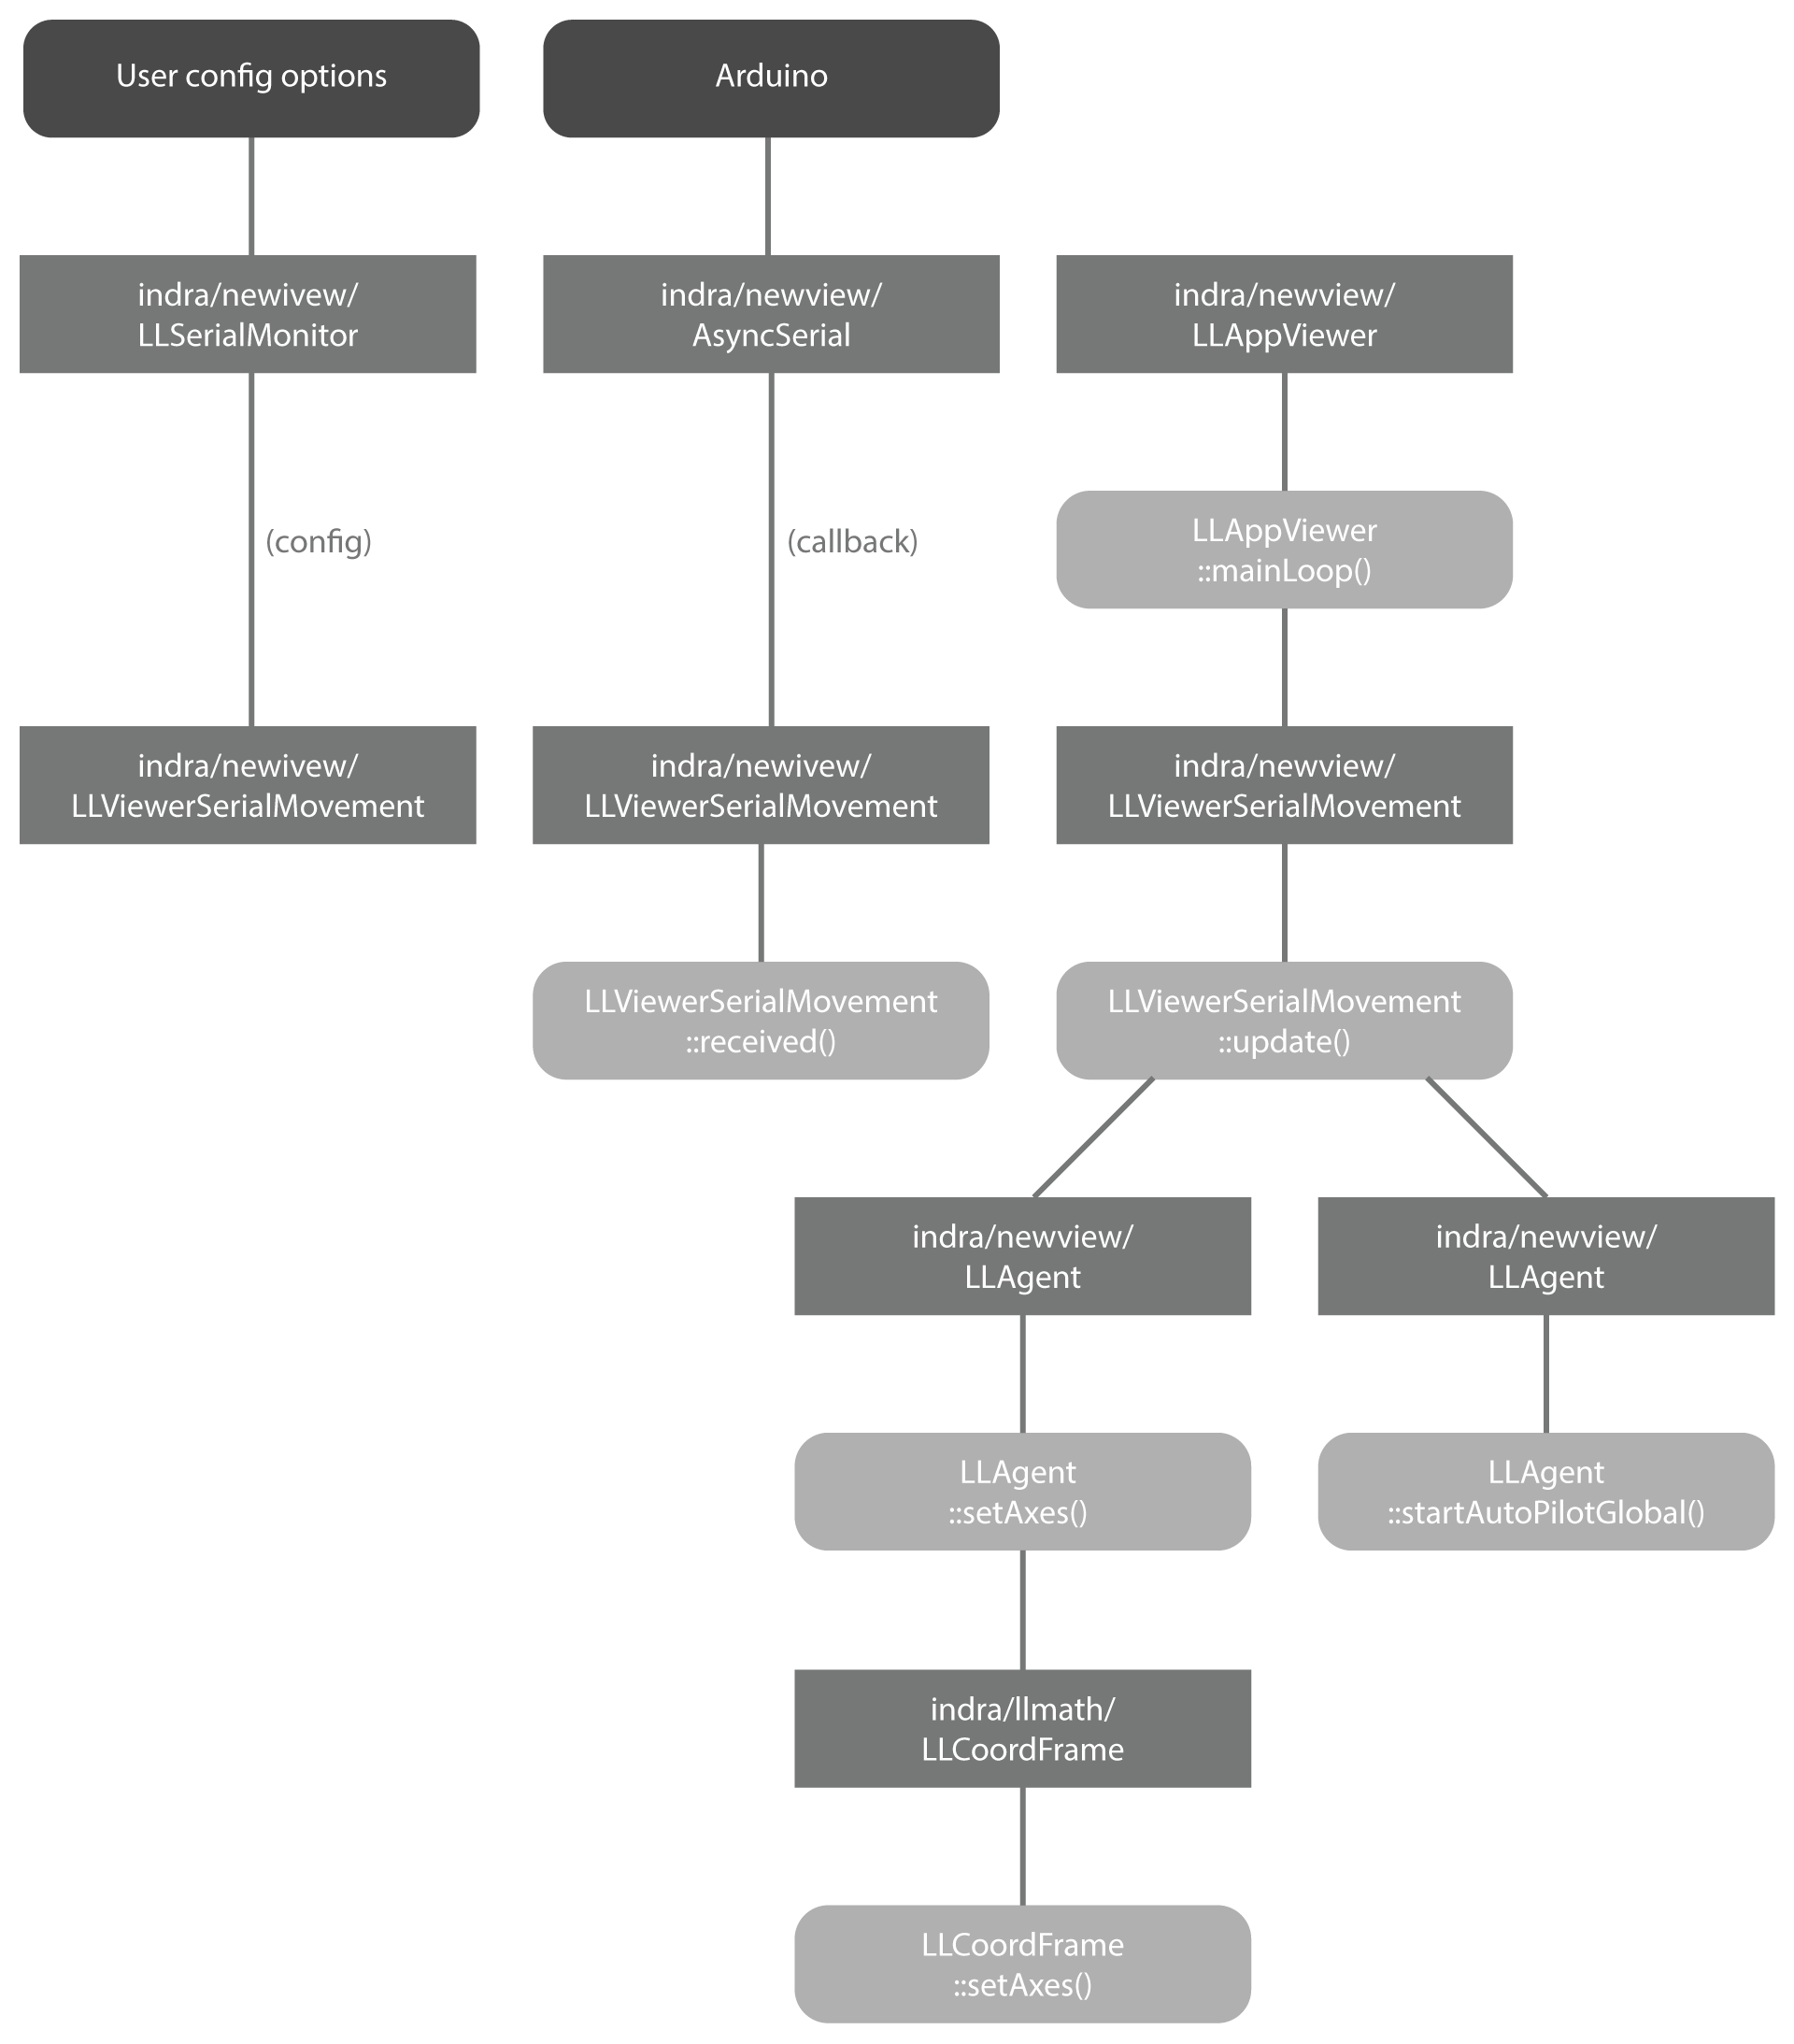
\includegraphics[width=.8\linewidth]{second_life_structure.png}
  \caption{Overview of modifications to Second Life client for VTW.}
  \label{second_life_structure.png}
\end{figure}

%=========================================================================================================

\subsection{\texttt{LLViewerSerialMovement} reference}
Table \ref{pangolin-function-reference} provides documentation of the functions in \path{/indra/newview/LLViewerSerialMovement}.
\begin{center}
\begin{longtable}{ p{4.2cm}  p{10cm} }

\toprule

\textbf{Function} & \textbf{Description} \\

\midrule

%=========================================================================================================
		
\texttt{::connect} & Safely connects to a serial device (if not already connected). \\
		
\midrule

%=========================================================================================================

\texttt{::disconnect} & Safely disconnects from a serial device (if already connected). \\
		
\midrule

%=========================================================================================================

\texttt{::received} & A callback method registered to the \path{CallbackAsyncSerial} class in \path{/indra/newview/AsyncSerial}. This function parses the data (\path{const} \path{char} \path{*data}) from the serial device, extracting complete messages to the variable \path{mostRecentMessage}. Because of the nature of the serial I/O, \path{*data} is not guaranteed to contain a discrete message from the Arduino containing both orientation and position data (it may contain a partial/incomplete message) thus this function has to parse the array and assemble discrete messages from multiple subsequent callbacks. \\
		
\midrule

%=========================================================================================================

\texttt{::update} & Called upon each iteration of \path{LLAppViwer::mainLoop()} and in turn calls \path{::updateFromMostRecentMessage()}, \path{::updateOrientation()} and \path{::updatePosition()}. \\
		
\midrule

%=========================================================================================================

\texttt{::updateFromMostRecent- Message} & Processes a complete message from the Arduino which has been assembled by \path{::received()} and extracts the constituent orientation and position values. \\
		
\midrule

%=========================================================================================================

\texttt{::updateOrientation} & Applies the orientation values extracted from an Arduino message to the avatar's camera. This is achieved by a call to \path{LLAgent::setAxes()} which calls \path{LLCoordFrame::setAxes()} in \path{/indra/llmath/LLCoordFrame}. The orientation values are passed as a quaternion, converting the bearing, pitch and roll values extracted from the Arduino message as degrees using \path{::quaternionFromDegrees()}.\\
		
\midrule

%=========================================================================================================

\texttt{::updatePosition} & Applies the position data extracted from an Arduino message to the avatar, using \path{LLAgent::startAutoPilotGlobal()} to perform smooth movement between the avatar's current position (obtained with \path{LLAgent::getPositionGlobal()}) and the new position derived from the Arduino (converted from latitude and longitude to Second Life region coordinates using \path{::latitudeLongitudeToRegionCoordinates()}). \\
		
\midrule

%=========================================================================================================

\texttt{::quaternionFromDegrees} & A helper method to convert a set of bearing, pitch and roll readings expressed separately in degrees, into a single quaternion. Quaternions are frequently used to represent rotations in 3D applications, as they do not suffer from gimbal lock; Second Life is no exception to this and internally uses quaternions for all rotation data, providing \path{/indra/llmath/LLQuaternion} for this purpose. \\
		
\midrule

%=========================================================================================================

\texttt{::latitudeLongitudeTo- RegionCoordinate} & Converts a real world position, expressed as a longitude and latitude pair, to the equivalent Second Life coordinates, applying the haversine formula using knowledge of the real world and corresponding Second Life position of the anchor point and the scale of the Second Life reconstruction compared to the real world. \\
		
\midrule

%=========================================================================================================

\texttt{::degreesToRadians} & A helper method to convert values expressed in degrees to the equivalent value expressed in radians (implementations of the haversine formula usually make use of radians). \\
		
\bottomrule

%=========================================================================================================

\caption{Reference of LLViewerSerialMovement functions.}
\label{pangolin-function-reference}
\end{longtable}
\end{center}

%=========================================================================================================

Controlling the avatar's position according to latitude and longitude readings from the GPS receiver was again implemented using the haversine formula. This implementation, included as figure \ref{secondlifehaversine}, can be compared to the OpenSim region module implementation previously included as figure \ref{RegionModuleCode1}. One important difference between this Second Life client implementation and the OpenSim region module implementation is that the former uses global coordinates, rather than local coordinates\regionmodulelimitationFootnote{}. This means that the Second Life client implementation allows positional control of an avatar across region boundaries, crucial for use with a cultural heritage reconstruction that spans multiple regions in an OpenSim `megaregion'\megaregionFootnote{} such as that used for evaluation of VTW.

These modifications to the Second Life client are configured/controlled via a window added to the client and accessed via a menu entry (see figure \ref{pangolin_second_life_dialogue.png}). The implementation of this window resides in \path{/indra/newview/LLViewerSerialMonitor}. This allows for specification of the path to the serial device, along with its baudrate, as well as the specification of the anchor point: the latitude and longitude of the point in the real world and the equivalent X/Y coordinates in the Second Life reconstruction. The window then provides diagnostic output showing the reconstructed messages coming in from the serial device, along with controls to individually enable/disable orientation and position control and alter the high-pass and smoothing applied to both controls.

\begin{figure}[h]
\centering
  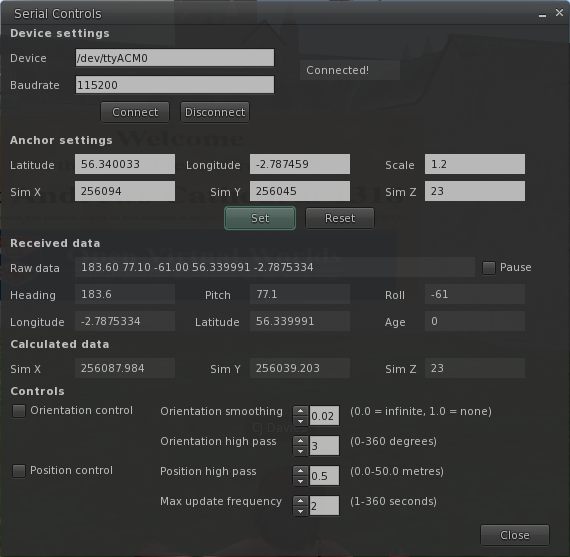
\includegraphics[width=0.6\linewidth]{pangolin_second_life_dialogue.png}
  \caption{Configuration window in VTW's modified Second Life client.}
  \label{pangolin_second_life_dialogue.png}
\end{figure}

\begin{figure}[h]
\begin{lstlisting}[language=C++, numbers=left, numberstyle=\small, stepnumber=1, frame=single, breaklines=true, backgroundcolor=\color{codebackground}, showstringspaces=false]
boost::tuple<float, float, float> LLViewerSerialMovement::latitudeLongitudeToRegionCoordinate(double newLat, double newLong, float anchorLat, float anchorLong, float scale, boost::tuple<float, float, float> anchorCoordinates) {

    double d, a, c, X, Y;

    // calculate difference in y (latitude) between anchor & new reading
    d = fabs(degreesToRadians(newLat - anchorLat));
    a = sin(d / 2) * sin(d / 2);
    c = 2 * atan2(sqrt(a), sqrt(1 - a));

    // mean radius of the Earth is 6371km (6371000m)
    d = 6371000 * c;

    // apply scale
    d *= scale;

    // sum appropriately from the anchor
    if (newLat > anchorLat) {
        Y = (anchorCoordinates.get<1>() + d);
    }
    else {
        Y = (anchorCoordinates.get<1>() - d);
    }

    // calculate difference in x (longitude) between anchor & new reading
    d = fabs(degreesToRadians((newLong - anchorLong)));
    a = sin(d / 2) * sin(d / 2) * cos(degreesToRadians(newLat)) * cos(degreesToRadians(anchorLat));
    c = 2 * atan2(sqrt(a), sqrt(1 - a));
    
    d = 6371000 * c;

    // apply scale
    d *= scale;

    // sum appropriately from anchor
    if (newLong > anchorLong) {
        X = (anchorCoordinates.get<0>() + d);
    }
    else {
        X = (anchorCoordinates.get<0>() - d);
    }

    return boost::make_tuple(X, Y, anchorCoordinates.get<2>());
}
\end{lstlisting}
\caption{Converting longitude and latitude to Second Life coordinates using haversine in modified Second Life codebase.}
\label{secondlifehaversine}
\end{figure}

%=========================================================================================================

\clearpage

%=========================================================================================================

\section{Evaluating VTW}

\newcommand{\thinkpadFootnote}{\footnote{\url{http://support.lenovo.com/us/en/documents/pd012148}}}

\newcommand{\wrtFootnote}{\footnote{\url{http://support.linksys.com/en-eu/support/routers/WRT54G}}}

%=====================

The site chosen for real world evaluation of the VTW platform was the impressive ruins of St Andrews cathedral.

\begin{figure}[h]
\centering
  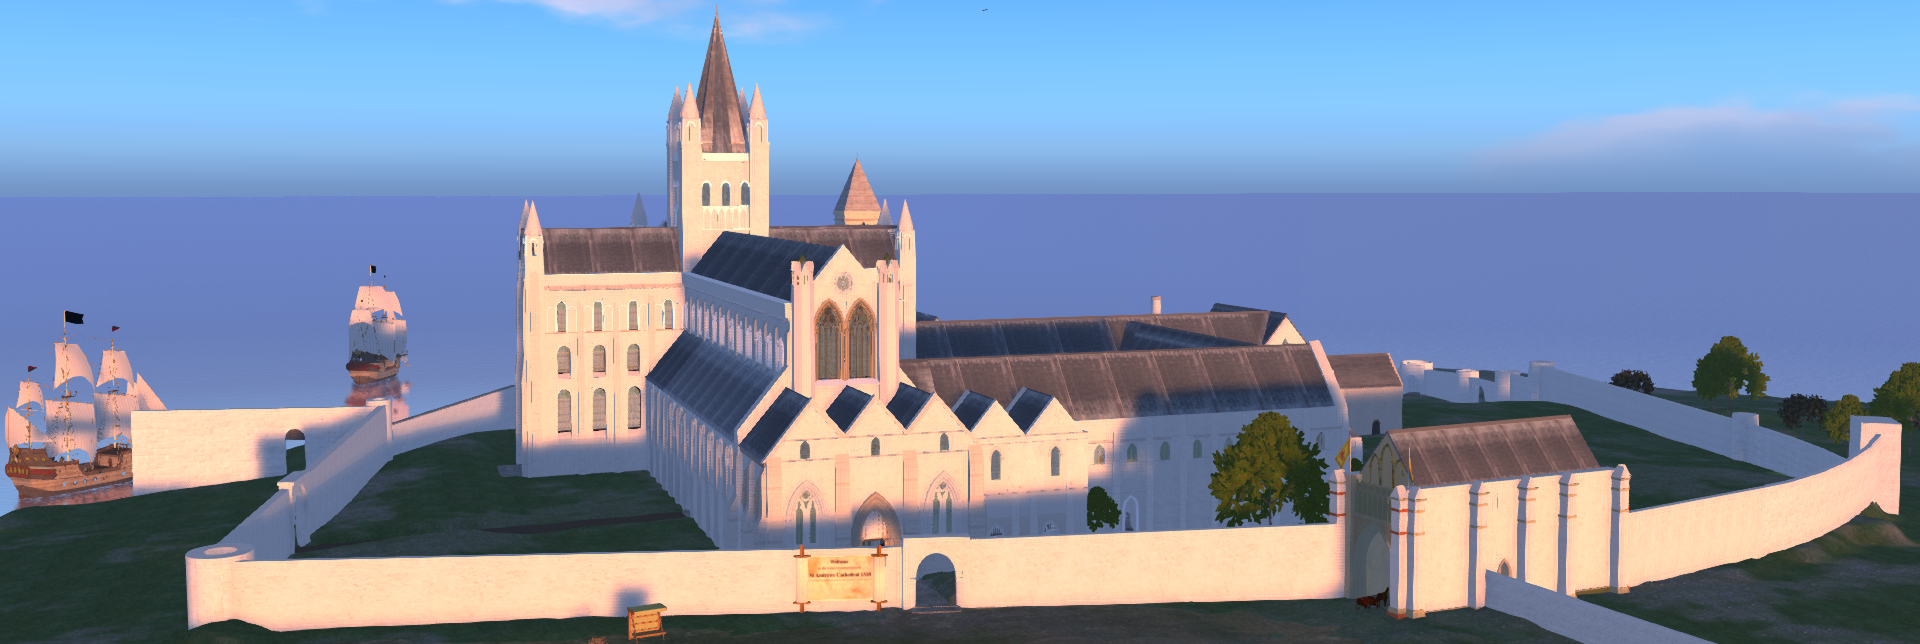
\includegraphics[width=\linewidth]{cathedral_reconstruction_side.png}
  \caption{St Andrews Cathedral reconstruction in Second Life/OpenSim, depicting the cathedral as it stood in 1318.}
  \label{cathedral_reconstruction_side.png}
\end{figure}

%=====================

%~\cite{Kennedy2013} Canons and Cathedrals

St Andrews Cathedral occupies a site used for worship since the 8th Century AD. Work on the Cathedral began around 1160 and was completed nearly 150 years later (the west fa\c{c}ade and parts of the nave collapsed in a storm around 1270). It was finally consecrated in 1318 four years after the battle of Bannockburn and in the presence of King Robert I of Scotland. In its prime, St Andrews Cathedral was the centre of Scotland's religious life, its largest and most magnificent church. In 1378 the Cathedral suffered a significant fire prompting
a reworking of many of its features, including the West and East End windows. Its presence was the catalyst for the foundation of the university at St Andrews in the early fifteenth century~\cite{Fawcett2011}. In 1561, following the Scottish reformation, the Cathedral was abandoned by the Bishops and replaced as the chief place of worship by the parish church. The cathedral was left to fall into ruin, with much of its stone being used in the construction of town dwellings.

%During its time the Cathedral was central to Scottish personalities and history: St Andrews was the highest ranking Scottish see. The establishment of Augustinian Cannons followed by the initiation of building work by Bishop Ernald reflected integration with the European church, economic dynamism and decline of the Celtic Church. The diocese funded Robert Bruce during the Wars of Independence. Its Bishop William de Lamberton contributed to the formulation of the Declaration of Arbroath, a central document in the formation of Scottish Nationhood. Isabella, sister of Donnchadh IV, last Pictish Earl of Fife, crowned Bruce King. John Knox personally lead his congregation against the Cathedral’s finery and following the murder of Cardinal Beaton the first Scottish protestant congregation was established in the Bishop’s palace.

Today the cathedral lies in ruins, but important fragments remain. The east gable of the presbytery, where the relics of St Andrew himself were purported to be kept, along with the south wall of the nave and the majestic West Entrance, all point to the Cathedral's former majesty. The cloister retains its ruined chapter house and stone-vaulted under crofts. Consequently much evidence of the Cathedral's form exists. A view from the present day taken from the nave looking towards the choir is shown by figure \ref{cathedral_real_outside.jpg}.

%=====================

The OVW Group's reconstruction of St Andrews cathedral, as shown in figures \ref{cathedral_reconstruction_side.png} and \ref{cathedral_reconstruction_above.jpg}, represents the site as it stood in 1318, the year of its consecration. This virtual reconstruction, presenting a historically accurate model of the cathedral as it stood at the peak of its former glory, is very large at over 400m by 600m and spanning multiple storeys.

\TwoFig{cathedral_real_outside.jpg} {St Andrews cathedral today.} {cathedral_real_outside.jpg}
       {cathedral_reconstruction_above.jpg} {St Andrews cathedral reconstruction.} {cathedral_reconstruction_above.jpg}

%=========================================================================================================

\subsection{Evaluation Process}

%Magnetic declination information was entered into the HMC6343 for the position of the cathedral and the date of our experiments. The HMC6343's hard-iron offset calculation feature was used each time the hardware configuration was altered. The sampling frequency of the HMC6343 was set to its highest value of 10Hz. Orientation was set to `upright front' to match the physical orientation of the IC in the experiments.


%The MAX-6 was operated in `pedestrian' dynamic platform model, use of SBAS correction data was enabled and frequency of readings was set to the maximum of 5Hz.

For the purposes of evaluating VTW at the cathedral, a temporary server and network setup was effected using a Lenovo ThinkPad X61s\thinkpadFootnote{} laptop computer to host the OpenSim server. This was connected to a Linksys WRT54G\wrtFootnote{} wireless router, powered from a 12V sealed lead-acid battery, to provide wireless communication between the OpenSim server and the WindPad over a much larger range than the laptop's internal wireless interface could provide. This setup is shown in use at the cathedral by figure \ref{pangolin_laptop_router_battery.jpg}, the architecture of this experimental implementation is shown by figure \ref{vtw_implementation.png} and figure \ref{vtw_in_use.jpg} shows VTW in use at the cathedral.

\TwoFig{pangolin_laptop_router_battery.jpg} {OpenSim Server and wireless AP used for VTW experiments.} {pangolin_laptop_router_battery.jpg}
       {vtw_in_use.jpg} {VTW in use at St Andrews cathedral.} {vtw_in_use.jpg}

\begin{figure}[h]
\centering
  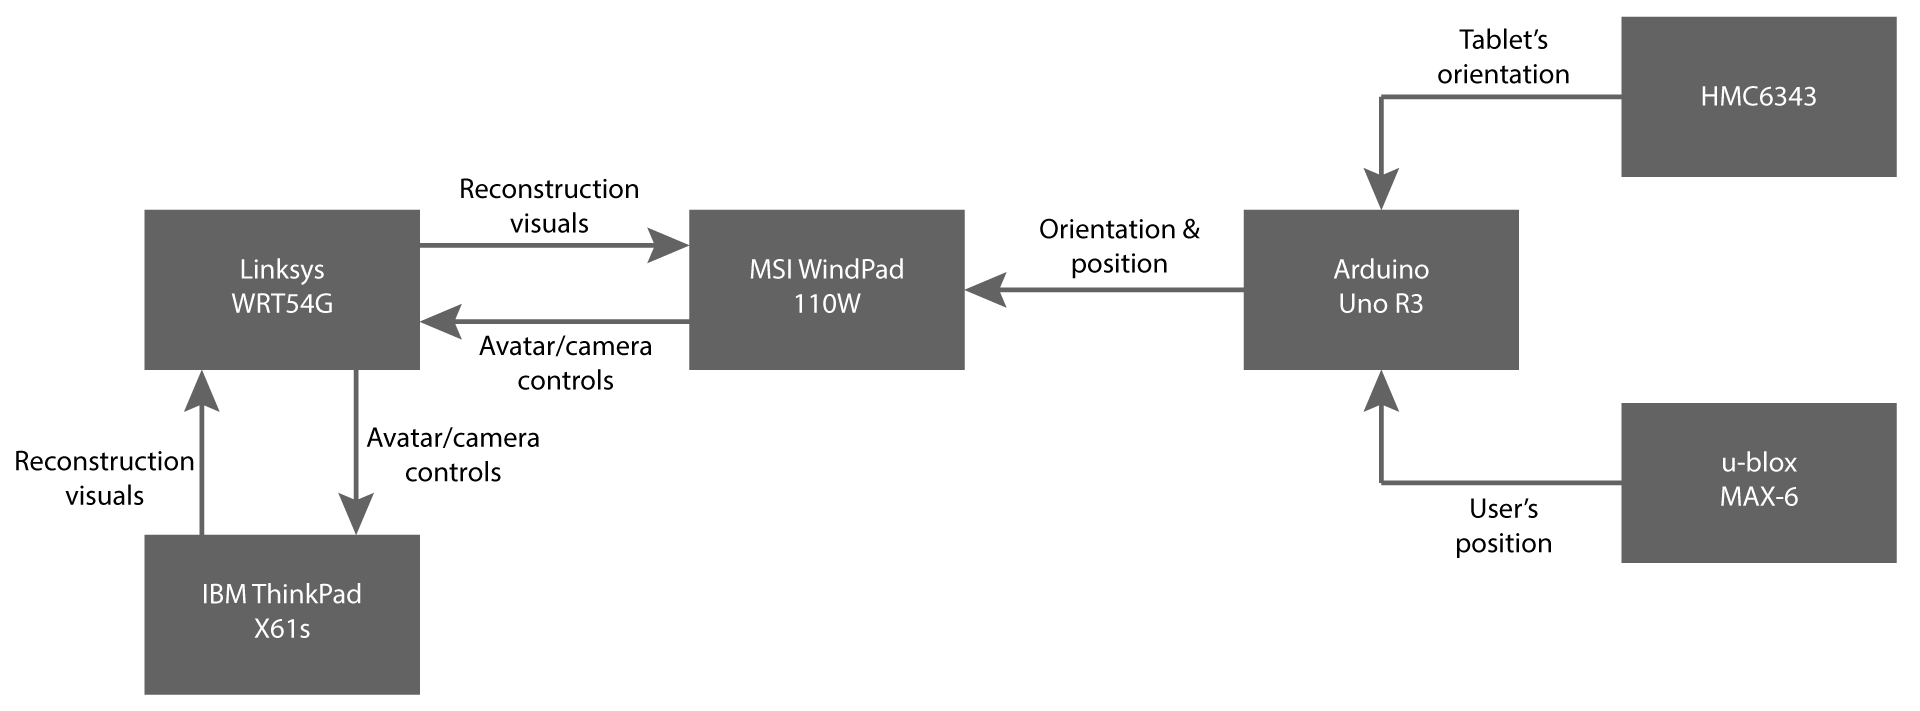
\includegraphics[width=\linewidth]{vtw_implementation.png}
  \caption{Architecture of VTW implementation during evaluation.}
  \label{vtw_implementation.png}
\end{figure}

%=========================================================================================================

\subsection{GPS Performance}

\newcommand{\ubloxcepFootnote}{\footnote{\url{https://u-blox.com/images/downloads/Product_Docs/MAX-6_ProductSummary_(GPS.G6-HW-10089).pdf}}}

\newcommand{\htconesFootnote}{\footnote{\url{http://www.htc.com/uk/smartphones/htc-one-s/}}}

\newcommand{\snapdragonFootnote}{\footnote{\url{https://www.qualcomm.com/products/snapdragon/processors/s4-s1}}}

\newcommand{\mytracksFootnote}{\footnote{\url{https://play.google.com/store/apps/details?id=com.google.android.maps.mytracks&hl=en}}}

\newcommand{\hausdorffFootnote}{\footnote{\url{http://postgis.net/docs/ST_HausdorffDistance.html}}}

%=====================

The product summary for the MAX-6 claims accuracy of 2.5m Circular Error Probable (CEP) without SBAS corrections and 2m CEP with SBAS corrections \textit{``demonstrated with a good active antenna''}\ubloxcepFootnote{}. This means that in an ideal situation with SBAS correction data available there is 50\% certainty that each position reported by the GPS receiver will be within 2m of its actual position. The SL-1202 antenna used by VTW is passive, however as the distance between antenna and the MAX-6 IC itself in the hardware application is only a few millimeters there would be negligible benefit from using an active antenna. Whether the SL-1202 constitutes `good' for achieving the headlining performance characteristics of the MAX-6 is debatable as the definition of `good' is not provided in the product summary.

To determine the real world accuracy attainable with the MAX-6 outfitted with the SL-1202 in the scenario of the cathedral as a cultural heritage site and thus which of the three scenarios outlined in section \ref{parallel-reality-in-virtual-heritage} the VTW platform could support, a route around the St Andrews cathedral ruins akin to the route that a visitor might take was planned. The route was walked with the MAX-6 connected to a laptop computer via an Arduino operating as a UART, feeding the raw NMEA messages into the u-center software version 7.0 which logged the messages for later evaluation. Simultaneously for comparative purposes a mid-range consumer Android smartphone was used to record the same track: a HTC One S\htconesFootnote{} containing a gpsOne Gen 8A solution within its Qualcomm Snapdragon S4 processor\snapdragonFootnote{}, using Google's My Tracks\mytracksFootnote{} app version 2.0.3 to record the data.

The three sets of positional data (planned route, MAX-6 recorded route and smartphone recorded route) were entered into a PostgreSQL database and the PostGIS database extender's \texttt{ST\_HausdorffDistance} algorithm\hausdorffFootnote{} was used to calculate the Hausdorff distances between the recorded routes and the planned route and between the recorded routes themselves. In this scenario, the Hausdorff distance represents the furthest distance needed to travel from any point on the route recorded by the GPS receiver to reach the nearest point on the planned route. Because of the substantially greater inaccuracies identified in the latter part of the recorded tracks, separate Hausdorff distances were calculated both for the complete tracks and also for truncated first and second sub-tracks.

%This ability to control navigation within the 3D virtual environment without explicit conscious input of keyboard/mouse/touch commands is integral to reducing the cognitive load required to maintain a presence within a virtual environment which is a key requirement for overcoming the vacancy problem and achieving successful mobile cross reality.

During the experiments the MAX-6 was unable to maintain reception of the additional correction data required for SBAS operation. When left stationary for several minutes reception was possible however subsequent movement of only a few meters at walking pace would reliably break reception. This reduced the theoretical maximum performance of the unit to 2.5m CEP, with observed performance being lower.

Figure \ref{vtw_all_routes.png} depicts an aerial view of the St Andrews cathedral ruins, oriented with North upwards; the blue line represents the planned route, red the route recorded by the MAX-6 receiver and green the route recorded by the smartphone while walking the planned route.

\begin{figure}[h]
\centering
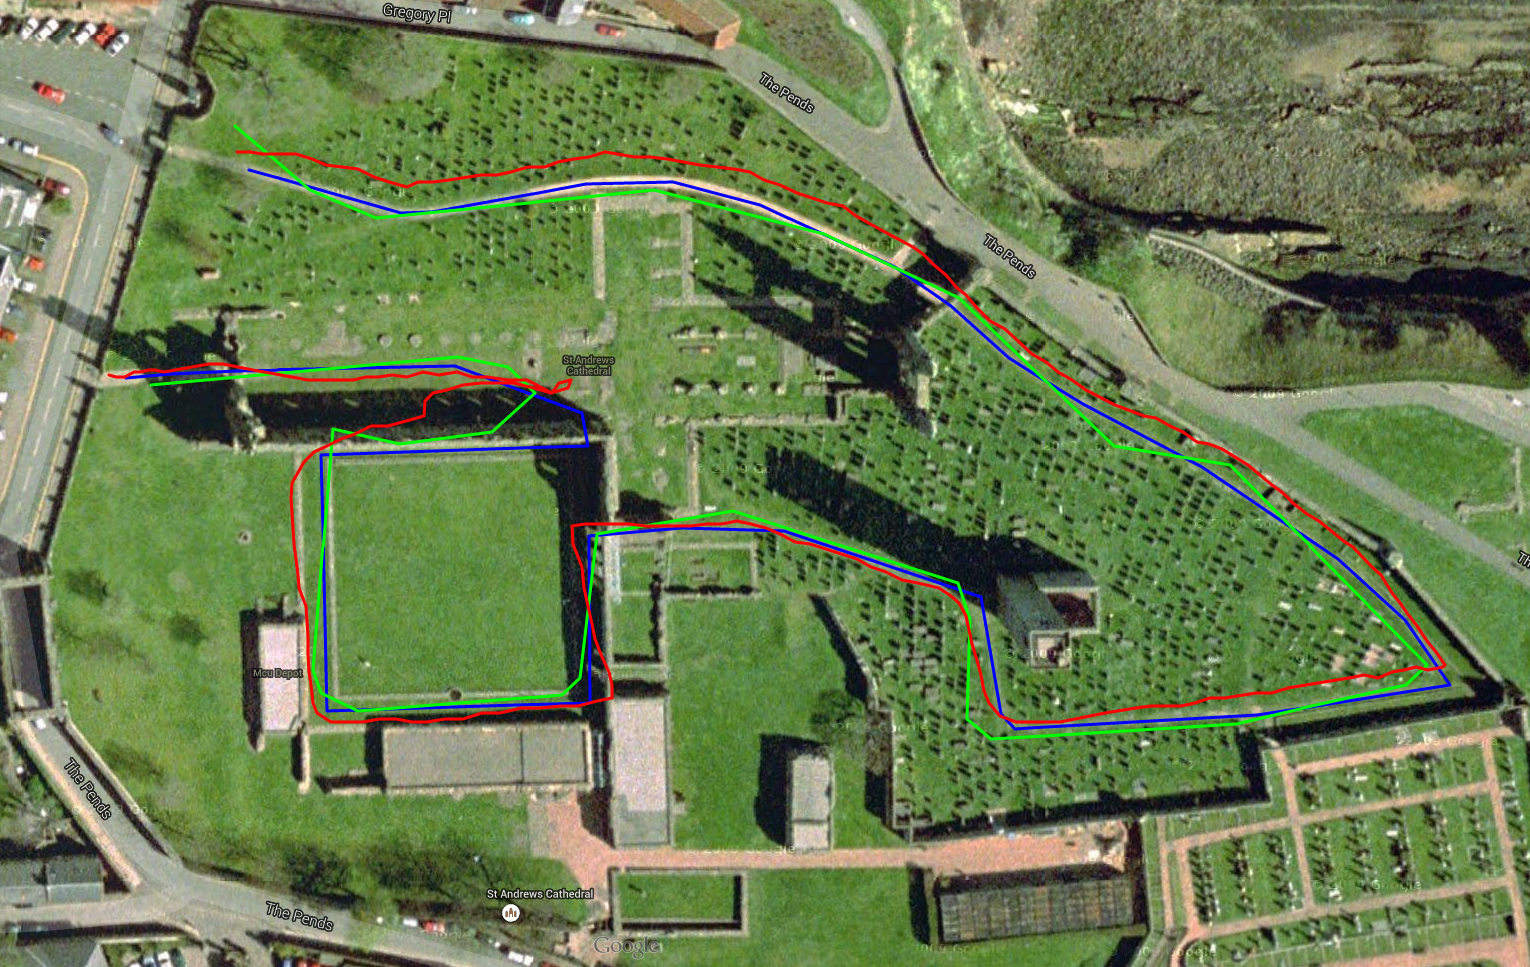
\includegraphics[width=0.8\textwidth]{vtw_all_routes.png}
\caption{Planned and recorded paths at St Andrews cathedral (complete track).}
\label{vtw_all_routes.png}
\end{figure}

The Hausdorff distance between the planned route and that recorded by the MAX-6 was $1.02e^{-04\circ}$. The `length' of a degree of latitude and a degree of longitude depends upon location upon the Earth; around the location of the St Andrews cathedral 1$^\circ$ of latitude is equivalent to 111347.95m and 1$^\circ$ of longitude to 61843.88m. Thus the Hausdorff distance of $1.02e^{-04\circ}$ can be visualized as $\pm11.3$m of North/South inaccuracy or $\pm6.3$m of East/West inaccuracy (or a combination of both N/S and E/W inaccuracy not exceeding a total displacement of $1.02e^{-04\circ}$ from the planned route).

The MAX-6 achieved better performance than the smartphone which recorded a Hausdorff distance of $1.33e^{-04\circ}$ ($\pm14.8$m N/S, $\pm8.2$m E/W). The Hausdorff distance between the routes logged by the MAX-6 and the smartphone was $1.14e^{-04\circ}$ ($\pm12.7$m N/S, $\pm7.0$m E/W) which represents a low correlation between the inaccuracies recorded by the two receivers even though they are of similar magnitudes from the planned route.

The maximum inaccuracies were recorded when walking along the South wall of the cathedral's nave. This wall is one of the most complete sections of the building with stonework reaching some 30ft above ground level (as can be seen in figure \ref{cathedral_real_outside.jpg} and in the shadows cast in figure \ref{vtw_all_routes.png}) which provides an effective obstruction to line-of-sight to half of the sky (and thus substantially impairing reception of signals from GPS satellites) when in proximity to it. This issue has been encountered in some earlier sitsim experiments~\cite{Liestøl2014}. When considering just the sub-track shown in figure \ref{vtw_alll_routes_first_half.png}, which terminates before this wall begins to significantly obstruct view of the sky, the Hausdorff distances are notably smaller; the MAX-6 achieved a Hausdorff distance of $7.23e^{-05\circ}$ ($\pm8.05$m N/S, $\pm4.47$m E/W), with the smartphone still behind with $8.99e^{-05\circ}$ ($\pm10.01$m N/S, $\pm5.56$m E/W). Again the Hausforff distance between the receivers showed low correlation between the inaccuracies, at $6.43e^{-05\circ}$ ($\pm7.12$m N/S, $\pm3.98$m E/W).
 
\begin{figure}[h]
\centering
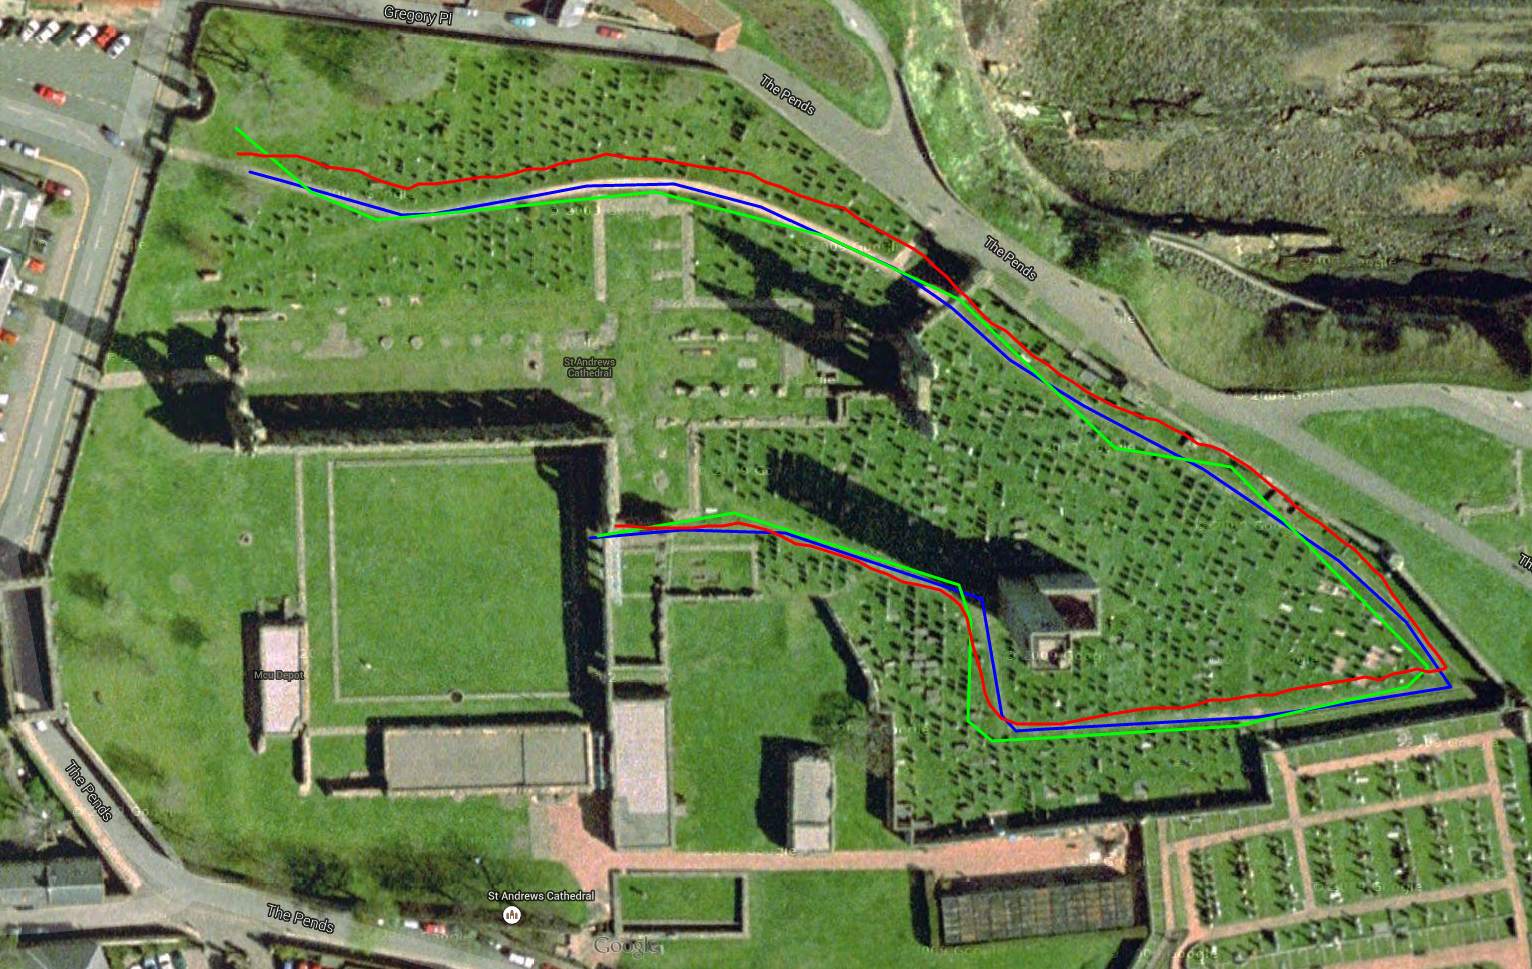
\includegraphics[width=0.8\textwidth]{vtw_alll_routes_first_half.png}
\caption{Planned and recorded paths at St Andrews cathedral (first sub track).}
\label{vtw_alll_routes_first_half.png}
\end{figure}

When analyzing the sub-track in the vicinity of the nave (see figure \ref{vtw_all_routes_second_half.png}) it can be seen that although the MAX-6 outperformed the smartphone in terms of Hausdorff distance this relationship is misleading as the smartphone track corresponded more closely in shape to the planned route even if it did stray further from it at its extreme. The discrepancy in the behavior of the two receivers in this situation is attributed to different implementations of dead-reckoning functionality between the receivers. Dead-reckoning is the process used when the GPS receiver loses reception of location data from satellites and extrapolates its position based upon a combination of the last received position data and the velocity of travel at the time of receiving these data (defined for the MAX-6 by the Dynamic Platform Model chosen).
 
\begin{figure}[h]
\centering
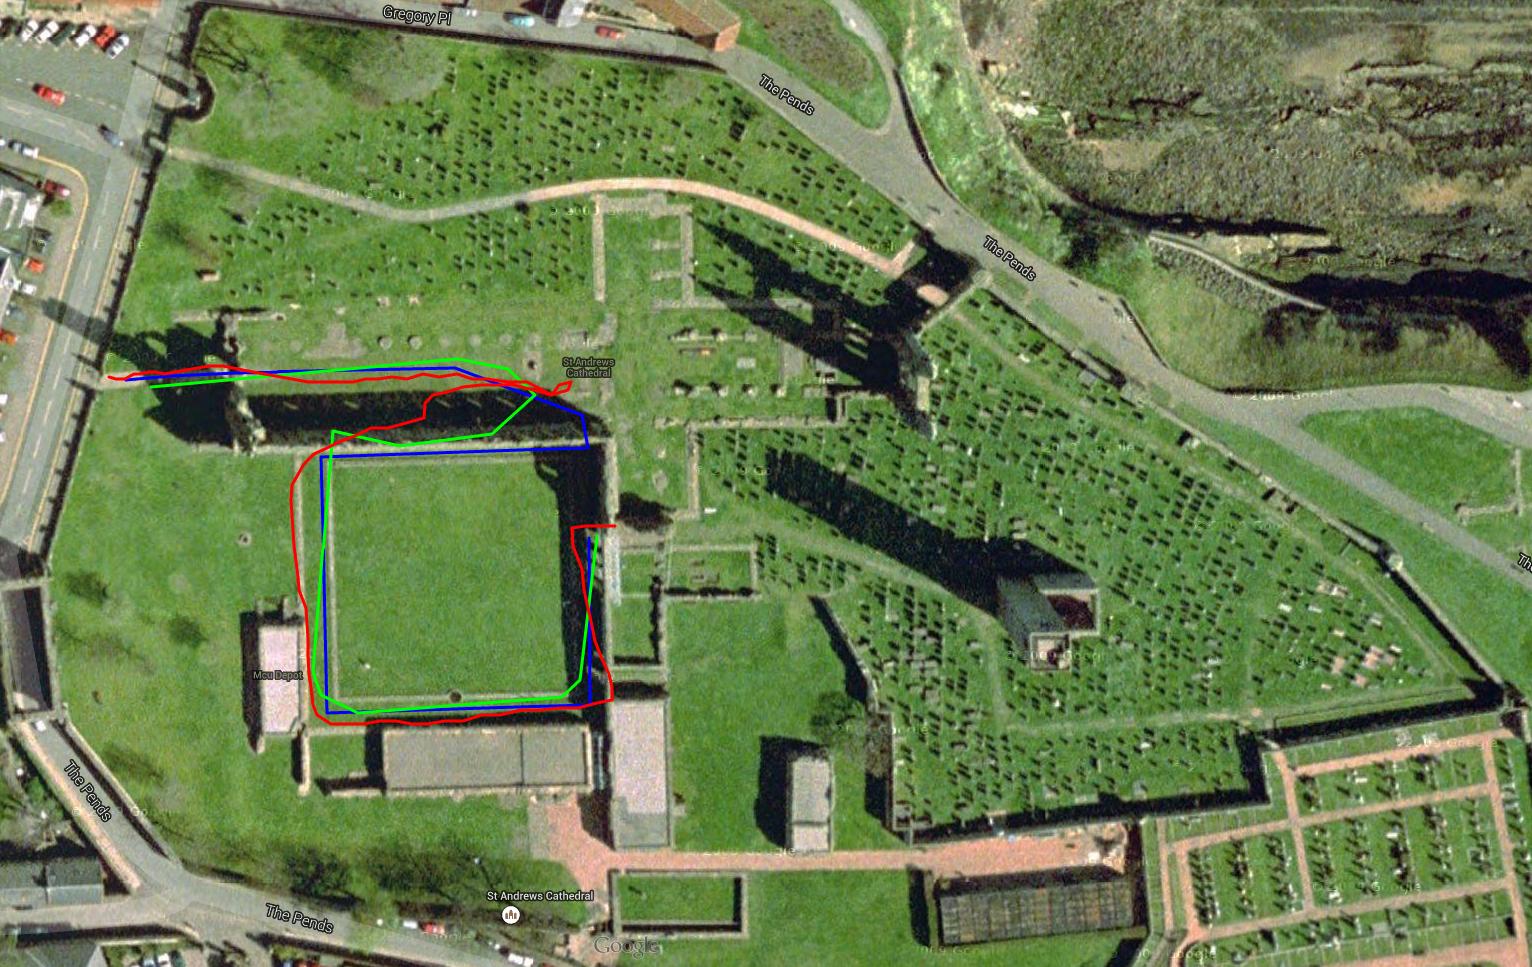
\includegraphics[width=0.8\textwidth]{vtw_all_routes_second_half.png}
\caption{Planned and recorded paths at St Andrews cathedral (second sub track).}
\label{vtw_all_routes_second_half.png}
\end{figure}

In addition to the accuracy of the position tracking it is also important to consider the frequency and granularity of these data. Even if the position data used by a freeform explorative parallel reality system were extremely accurate, the experience of using that platform would be poor if these data were reported too infrequently, as it would either lead to `jumpy' movement where the virtual view had to move a substantial distance to match each newly reported real position, or a reliance upon dead-reckoning to predict the user's movement between subsequent data. Likewise even with accurate and frequently reported position data, if the granularity of these data is not especially fine then the experience of using the platform will be negatively impacted by an inability to make small real movements and see them reflected as similarly small virtual movements when trying to pay attention to specific aspects of the environments.

Throughout the test route the HTC One S only reported 27 positions. This would have resulted in extremely large virtual movements if used for VTW and the low granularity of these positions (as seen in figure \ref{vtwpositiondeltas.png}) would have meant that the user would've found it frustratingly difficult to match real world movements to virtual world equivalents in any sort of freeform exploration scenario. The MAX-6 performed substantially better in these regards, reporting 251 positions along the same route and with substantially higher granularity (also shown in figure \ref{vtwpositiondeltas.png}).

However when the MAX-6 readings were integrated into the VTW platform and it was tested in its complete form at the cathedral, even though subsequent positions reported by the MAX-6 were usually no more than 1-3m away, they did not `settle' and keep the virtual view in the same position when standing still. Instead new readings in this 1-3m range would continue to be reported and the virtual view would continue to move even while the user was standing stationary in the real world. Adjusting the high pass filter on incoming position data to remedy this situation led to a worse experience when moving, as virtual position would only update in jumps of multiples of the high pass value.

\begin{figure}[h]
\centering
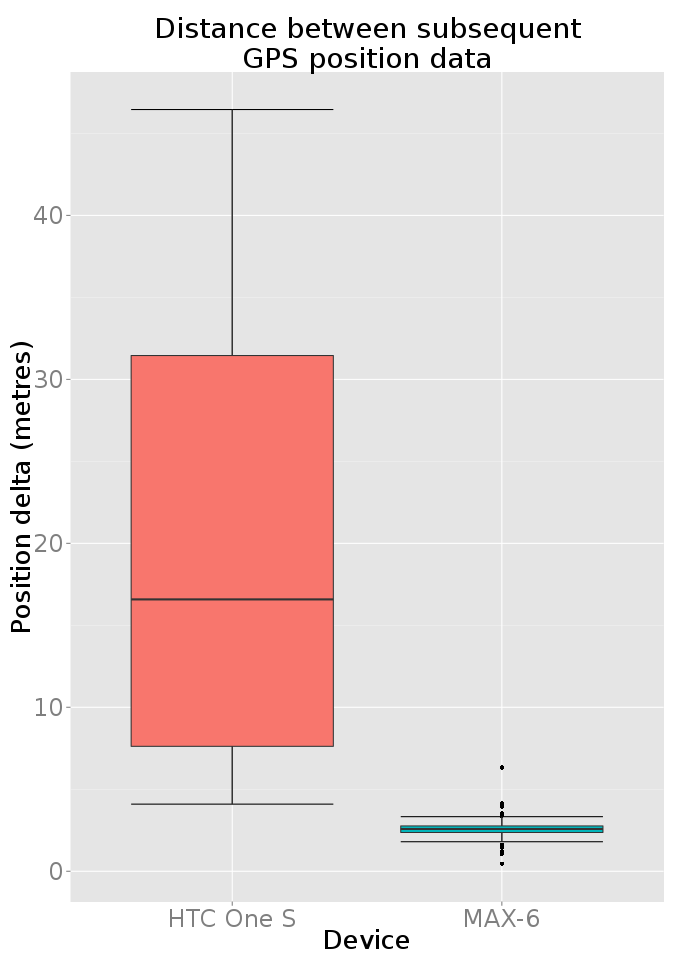
\includegraphics[width=0.5\textwidth]{vtwpositiondeltas.png}
\caption{Distance between subsequent GPS position data.}
\label{vtwpositiondeltas.png}
\end{figure}

%=========================================================================================================

%VTW's camera control from orientation data does not have as stringent performance criteria as its movement control. Unlike augmented reality applications where sparse virtual content is superimposed upon a view of a real environment and the virtual objects must be placed accurately in order for the effect to work well, parallel reality presents a complete virtual environment that in the case of VTW is viewed alternately side-by-side with the real environment and thus discrepancies between orientation of real and virtual environments has a less detrimental effect.

%=========================================================================================================

\subsection{Graphical Performance}

VTW averaged framerates between 20 and 25 frames per second (fps) with the modified Second Life client's quality option set to the `Low' position during testing at the cathedral site. Figure \ref{vtw-framerates.png} shows average framerates of the client's different quality options when standing at two different positions within the cathedral site; one `indoor' position from the centre of the nave and one `outdoor' position from the grassy area surrounded by the cloisters. The framerates for the indoor position were lower than those for the outdoor position as the virtual cathedral model features substantially more detail indoors than outdoors, due to the number of furnishings, tapestries, etc. that originally filled the building and which have been faithfully reconstructed in the virtual model.

\begin{figure}[h]
	\centering
	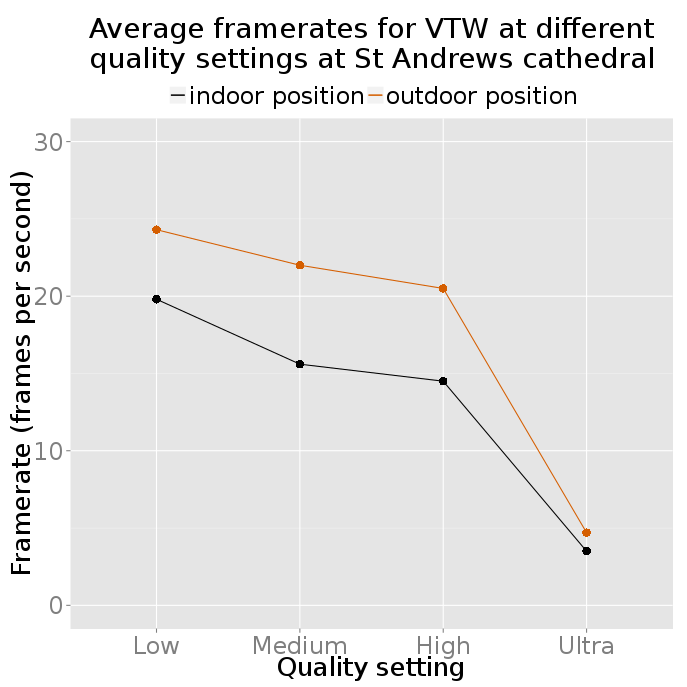
\includegraphics[width=0.5\textwidth]{vtw-framerates.png}
	\caption{Average framerates for VTW at St Andrews cathedral.}
	\label{vtw-framerates.png}
\end{figure}

The style of explorative interaction with virtual content that the VTW platform employs is more resilient to lower frame rates than other scenarios of interaction with virtual content such as fast paced competitive video games including first person shooters [20], but overall user experience would nonetheless have been improved by a higher frame rate. It should however be noted that the cathedral reconstruction was created with relatively powerful desktop computers in mind as the primary deployment platform and was not optimized for use on less powerful mobile platforms such as the tablet used by VTW.

The accuracy of the camera control during testing was sufficient, however the speed at which the camera orientation moved to match physical orientation was rather slow, resulting in having to wait for the display to `catch up' to changes in orientation. This is attributed to the 10Hz sampling rate of the orientation sensors which, particularly after readings were combined for smoothing purposes to reduce jerky movement, resulted in too infrequent orientation updates.

%=========================================================================================================

\subsection{Performance Implications}

When considering the Hausdorff distance of $1.02e^{-04\circ}$ in relation to the three scenarios outlined in section \ref{parallel-reality-in-virtual-heritage} it is important to remember that this figure represents the worst case scenario and is not necessarily a good indication of average performance. This value, analogous to $\pm11.3$m of North/South inaccuracy or $\pm6.3$m of East/West inaccuracy, represents a constraint on the granularity of the content; it is the minimum distance required between any two points to guarantee that they are correctly differentiated between, however it does not mean that two points separated by less than this distance will \textit{never} be correctly differentiated between.

Considering the first scenario of static viewpoints this level of positional accuracy is plenty sufficient and the value of $1.02e^{-04\circ}$ can be used in the selection process to ensure that viewpoints are spaced sufficiently that there is no chance for incorrect identification of the current viewpoint.

Considering the second scenario of freeform exploration, this level of positional accuracy is not ideal but was still sufficient during the evaluation to explore certain areas of the cathedral site in this unrestricted fashion. Whilst accuracy of this level is not sufficient to reliably differentiate between two adjacent rooms or to allow a user to `walk through' a virtual doorway nor to examine an object closely when standing still, due to the manner in which the position data did not `settle', when considering a large site such as the cathedral at which visitors are often viewing the site from some distance due to its sheer size this level of accuracy is sufficient for some freeform exploration. For example when walking on the central grass area enclosed by the cloisters (the large square area seen toward the bottom left of figures \ref{vtw_all_routes.png} through \ref{vtw_all_routes_second_half.png}) and using VTW to look North/East toward the virtual cathedral proper (a situation shown in figure \ref{vtw_in_use.jpg}), the positional discrepancy was largely imperceptible - when looking at the cathedral building from 50m away, a discrepancy of 5m did not seem to pose any problem. It is only when approaching features more closely that the discrepancy between real and virtual becomes apparent, a relationship observed by Wither et al. when experimenting with indirect augmented reality.

\begin{quote}
	\textit{``Our user study results suggest that Indirect AR does very well in outdoor applications where the user is more than a few meters away from the physical objects of interest.''}~\cite{Wither2011}
\end{quote}

Considering the third scenario with detailed comparison of objects and artefacts in close proximity is where the positional discrepancy of VTW and its tendency not to settle renders the experience unworkable. When walking from the cloisters through the real South wall into the cathedral nave, the virtual vantage would pass through the virtual South wall several metres to one side of the virtual doorway. Comparison between an object the size of a doorway from a distance of a few meters in the manner that scenario 3 envisages would be unworkable in this manner.

%The accuracy of orientation tracking does not change with different positional accuracy and the accuracy attained in the experiments was sufficient for an acceptable user experience, however the experience would benefit from better graphical quality and higher responsiveness to changes in user orientation.

%=========================================================================================================

\subsection{Real World Experience of VTW}
\label{real-world-experience-of-vtw}

%How with VTW we have a small `window' into the virtual, which is then surrounded by the real. So unlike Mirrorshades which is about distributing attention by time (one environment, then the other), VTW is about distributing attention by gaze/place (different parts of a single view/combined environment).

Revisiting the definition of parallel reality (section \ref{parallelrealityinbackground}), one can consider it to be distinguished by two principal features:

\begin{enumerate}
	\item The environmental aspect - are there two complete environments, one real and the other virtual?
	\item The experiential aspect - can the user freely switch between the environments?
\end{enumerate}

Although the VTW platform was developed with investigation of the parallel reality concept in mind and definitely fulfils the environmental aspect of the definition by presenting complete real and virtual environments to the user, the experience of using the system at St Andrews Cathedral fell somewhat short of the vision for the experiential aspect of the definition. Instead of \textit{switching} between the two complete environments, the virtual environment in VTW was instead seen as a window within the wider real environment. Even when focussing attention upon the virtual environment via the device's screen, one also perceived the real environment around it, filling the majority of the viewport, due to the greater `peripheral view'~\cite{Billinghurst2014} that the handheld interface presents compared to a HMD. The experience was more of \textit{mixing} (even if that mixing was performed by the human mind and not by the device itself), distributing attention by gaze, rather than \textit{switching} to a complete/discrete environment at the exclusion of the other, distributing attention by time.

Both with previous sitsim projects and VTW the user's view is arguably always a mix, never purely virtual, and the user's position upon the locus of attention axis of the combined Milgram/Waterworth model can never reach its virtual extreme, due to the fact that the screen is always seen as a part of the larger real environment. This was a consideration in section \ref{the-virtual-time-window}, however it was only upon experiencing the platform first hand that the extent of this situation could be comprehended. This similarity in experience between VTW and traditional augmented reality platforms may clarify how from the point of view of user experience, sitsim projects have been labelled in the past as indirect augmented reality, even if from the point of view of the environments that they provide, they are distinct.

%=========================================================================================================

\section{Summary}

This chapter has introduced virtual heritage as a field in which the application of alternate reality techniques has a demonstrated history of success and to which the application of parallel reality promises to be of further benefit. The Virtual Time Window project was a preliminary foray into the application of parallel reality to virtual heritage, making use of an x86 tablet computer imbued with position and orientation sensing via GPS and accelerometer/magnetometer, for tandem exploration of outdoor cultural heritage sites and their virtual reconstructions by leveraging existing OpenSim content. VTW assessed via real world application the suitability of an interface in the style of previous sitsim projects to serve as a platform for investigation into parallel reality experience. This real world experimentation revealed that while the accuracy of positional tracking obtainable by the discrete GPS receiver of the VTW platform was sufficient both for a scenario in which the user observes the virtual environment at static viewpoints and for a level of freeform exploration wherein a certain distance is maintained between the user and the objects being observed, the experiential aspect of the system was not as novel when compared against previous augmented reality and sitsim projects as the concept of parallel reality envisioned.

%=========================================================================================================